\documentclass[a4paper,10pt]{article}
\usepackage[utf8]{inputenc}

% ----  Useful packages % ---- 
\usepackage{amsmath}
\usepackage{graphicx}
\usepackage{amsfonts}
\usepackage{amsthm}
\usepackage{amssymb}
% ----  Useful packages % ---- 

\usepackage{wrapfig}
\usepackage{caption}
\usepackage{subcaption}

\graphicspath{ {./images/} }

% ---- Set page size and margins replace ------
\usepackage[letterpaper,top=2cm,bottom=2cm,left=3cm,right=3cm,marginparwidth=1.75cm]{geometry}
% ---- Set page size and margins replace ------

% ---- Definition of custum section ---- 
\newtheorem{note}{Note}[subsection]
\newtheorem{definition}{Definizione}[section]

\theoremstyle{definition}
\newtheorem{example}{Esempio}[section]

% ------- OSSERVAZIONE ------
\theoremstyle{definition}
\newtheorem{observation}{Osservazione}[subsection]
% ------- OSSERVAZIONE ------

\theoremstyle{definition}
\newtheorem{demostration}{Dimostrazione}[section]

\theoremstyle{plain}
\newtheorem{theorem}{Teorema}[section]
% ---- Definition of custum section ---- 

% ---- Footer and header ---- 
\usepackage{fancyhdr}
\pagestyle{fancy}
\fancyhf{}
\fancyhead[LE,RO]{A.A 2022-2023}
\fancyhead[RE,LO]{Programmazione ed Algoritmi}
\fancyfoot[RE,LO]{\rightmark}
\fancyfoot[LE,RO]{\thepage}

\renewcommand{\headrulewidth}{.5pt}
\renewcommand{\footrulewidth}{.5pt}
% ---- Footer and header ---- 

% ----  Language setting ---- 
\usepackage[italian, english]{babel}
% ----  Language setting ---- 

\usepackage{listings}
\usepackage{color}
\definecolor{lightgray}{rgb}{1,1,1}
\definecolor{darkgray}{rgb}{.4,.4,.4}
\definecolor{purple}{rgb}{0.65, 0.12, 0.82}

\lstdefinelanguage{JavaScript}{
  keywords={typeof, new, true, false, catch, function, return, null, catch, switch, var, let, ref, if, in, while, do, else, case, break},
  keywordstyle=\color{blue}\bfseries,
  ndkeywords={class, export, boolean, throw, implements, import, this, print},
  ndkeywordstyle=\color{darkgray}\bfseries,
  identifierstyle=\color{black},
  sensitive=false,
  comment=[l]{//},
  morecomment=[s]{/*}{*/},
  commentstyle=\color{purple}\ttfamily,
  stringstyle=\color{red}\ttfamily,
  morestring=[b]',
  morestring=[b]"
}

\lstset{
   language=JavaScript,
   backgroundcolor=\color{lightgray},
   extendedchars=true,
   basicstyle=\footnotesize\ttfamily,
   showstringspaces=false,
   showspaces=false,
   numbers=left,
   numberstyle=\footnotesize,
   numbersep=9pt,
   tabsize=2,
   breaklines=true,
   showtabs=false,
   captionpos=b
}

\usepackage{multicol}

\usepackage{hyperref}
\hypersetup{
	colorlinks,
	citecolor=black,
	filecolor=black,
	linkcolor=black,
	urlcolor=black
}

\title{\textbf{Programmazione ed Algoritmi}}
\author{Realizzato da: Giuntoni Matteo e Ghirardini Filippo}
\date{A.A 2022-2023}

\begin{document}
\maketitle
\newpage
\tableofcontents

\section{Introduzione}

\subsection{Insiemi Numerici}
Un insieme di numeri è una raccolta di elementi. Alcuni degli insiemi che verranno utilizzati maggiormente in questo corso sono:
\begin{itemize}
    \item \textbf{N. Naturali} cioè tutti gli interi non negativi: $\mathbb{N}$ = $\{0, 1, 2, 3, 4, ...\}$.
    \item \textbf{N. Interi} cioè tutti gli interi con segno qualsiasi: $\mathbb{Z} = \{..., -3, -2, -1, 0, 1, 2, 3, ...\}$.
    \item \textbf{N. Razionali}, cioè le frazioni: $\mathbb{Q} = \{\frac{p}{q}$ dove p e q $\in \mathbb{Z}$ e $q \neq 0\}$. \\
    Un sottoinsieme sono le \textbf{classi di equivalenza} che sono tutte le frazioni semplificate ai minimi termini. 
    \item \textbf{N. Reali}, che possono essere visti come tutti gli elementi rappresentabili su una retta: $\mathbb{R}$ 
\end{itemize}
\begin{note}
I vari insiemi si contengono fra di loro. ($\mathbb{N} \subset \mathbb{X} \subset \mathbb{Q} \subset \mathbb{R}$) 
\end{note}
\begin{note}
Esistono molti numeri reali che non sono razionali e non si possono scrivere come frazioni. E.g. $\sqrt{2}, \pi, ...$
\end{note}

\subsection{Intervalli}
\begin{definition}[Intervallo]
    Un sottoinsieme $I \subseteq \mathbb{R}$ è un intervallo se $\forall \: x,\:y \in I$ $\mid$ $x < y$ $\wedge$ $\forall z \mid x < z < y$ ho che $z \in I$. [\ref{fig:intervallo}]
\end{definition}
\begin{wrapfigure}{l}{7cm}
	\vspace{-20pt}
	\centering
	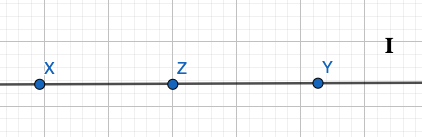
\includegraphics[width=5cm]{Intervallo.png}
	\caption{Tutto il segmento fra x e y deve stare in I}
	\label{fig:intervallo}
\end{wrapfigure}
I è un intervallo se ogni \emph{ogni} punto che prendo tra gli estremi dell'intervallo, questo appartiene all'intervallo stesso.
\\\\\\\\\\
\begin{example}
Esempi di intervalli.\\ \\
Questo caso \textbf{è un intervallo} \hspace{3.2cm} Questo caso \textbf{non è un intervallo} fra A e D.
\begin{figure}[h!]
    \vspace{-10pt}
    \begin{subfigure}{.5\textwidth}
        \hspace{-50pt}
        \centering
        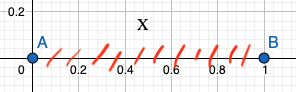
\includegraphics[width=6cm]{Esempio-intervallo-1.png}
        \caption{$A = \{x \in \mathbb{R} \: | \: 0<x<1\}$}
    \end{subfigure}
    \begin{subfigure}{.5\textwidth}
        \centering
        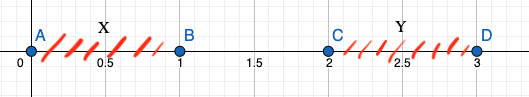
\includegraphics[width=7.5cm]{Esempio-intervallo-2.png}
        \caption{$C = \{x \in \mathbb{R} \: | \: 0<x<1 \: \vee \: z<x<3\}$}
    \end{subfigure}
\end{figure}
\end{example}

\newpage
\subsection{Notazione}
Con $a, b \in \mathbb{R}$ e con $a < b$ è possibile scrivere le notazioni in tabella \ref{tab:notazione-intervalli}.
\begin{table}[h!]
    \centering
    \setlength{\tabcolsep}{7pt}
    \renewcommand{\arraystretch}{2}
    \begin{tabular}{|c|c|c|} \hline
        [a, b] & Intervallo chiuso di estremi a e b & $\{x \in \mathbb{R} \: | \: a \leq x \leq b\}$ \\ \hline
        (a, b) & Intervallo aperto & $\{x \in \mathbb{R} \: | \: a < x < b\}$ \\ \hline
        [a, b) & Intervallo semi aperto a destra & $\{x \in \mathbb{R} \: | \: a \leq x < b\}$ \\ \hline
        (a, b] & Intervallo semi aperto a sinistra & $\{x \in \mathbb{R} \: | \: a < x \leq b\}$ \\ \hline
        [a, $+\infty$) & Semiretta chiusa a sinistra & $\{x \in \mathbb{R} \: | \: a \leq x\}$ \\ \hline
        ($-\infty$, b] & Semiretta chiusa a destra & $\{x \in \mathbb{R} \: | \: x \leq b\}$ \\ \hline
        ($-\infty$, $+\infty$) & Insieme di tutti i numeri $\mathbb{R}$ & $\{x \in \mathbb{R}\}$ \\ \hline
    \end{tabular}
    \caption{Notazione Intervalli}
    \label{tab:notazione-intervalli}
\end{table}
\newpage
\section{Array}
Una struttura dati molto conosciuta e chiamata array.
\begin{definition}[Array]
Gli array sono delle strutture dati omogenea, statiche e lineari implementate mediante un gruppo di celle contigue di memoria dello stesso tipo.
\end{definition}

Di seguito due esempi grafici di array uno di interi ed uno di stringhe, da notare sotto la posizione degli elementi nell'array che si conta partendo dallo 0.
\begin{figure}[h!]
    \centering
    \begin{subfigure}{.5\textwidth}
        \centering
        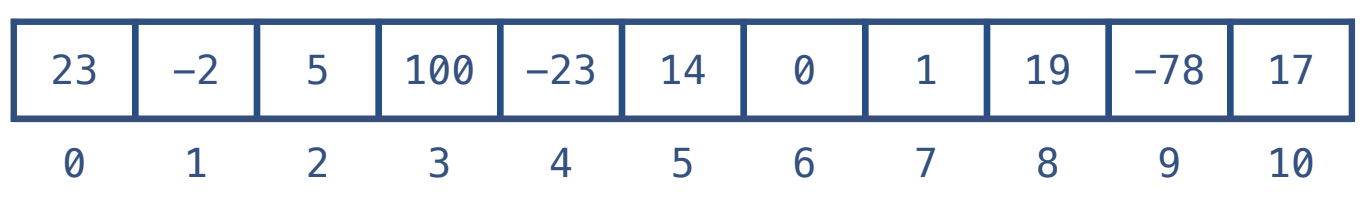
\includegraphics[width=9cm]{images/esempio-array-1.png}
        \caption{}
    \end{subfigure}
    \hfill
    \begin{subfigure}{.4\textwidth}
        \centering
        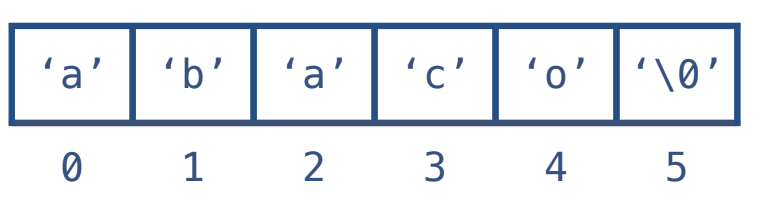
\includegraphics[width=6cm]{images/esempio-array-2.png}
        \caption{}
    \end{subfigure}
    \caption{In (a) un array lungo 11 di interi, in (b) un array lungo 6 di caratteri}
\end{figure}
\begin{note}
Nota che nell'array di caratteri sopra nell'ultima posizione c'è sempre $\setminus0$ (Null).
\end{note}
Negli array si accede mediante l'indice della posizione nella sequenza. Si possono inoltre effetturare sugli elementi tutte le operazioni definte sul tipo corrispondete agli elementi dell'array.
\begin{example}
Alcuni esempi di accesso ed operazioni su gli arrey sopra:
\begin{itemize}
    \item a[6] == 0 \hspace{.5cm} a[3] == 100 \hspace{.5cm} b[2] == 'a' 
    \item a[4] = a[5] + a[7] \: \: (a[5] == 14, a[7] == 1, quindi il risultato sarà 14 + 1 = 15)  
\end{itemize}
\end{example}

Inoltre possiamo dire che gli array sono allocati in memoria quando il controllo del flusso a tempo di esecuzione entra nel blocco in cui sono definiti e sono distrutti quando il controllo esce dal blocco.\\\\
Il nome dell'array è una variabile che contiene la locazione di memoria in cui è memorizzata la prima cella. Essendo che le celle sono contigue e hanno tutte lo stesso tipo basta infatti conoscere la posizione della prima cella per poi, tramite una semplice operazione algebrica di somma, accedere a quelle successive. In generale possiamo scrivere che:
\begin{center}
    $a[i] \: \: = \: \: \sigma(\rho(a) + size(type(a)) \times i)$
\end{center}
\begin{example}
Se abbiamo un array di lunghezza 11, ed chiamiamo la prima locazione (quella dove è contenuto il primo elemento dell'array) loc1, per raggiungere la posizione numero 10 basterà eseguire l'operazione loc1 + 32*10.
\end{example}
Questo consente l'accesso diretto agli elementi degli array con una sola operazione indipendentemente dalla lunghezza dell'array (consto di accesso costante). 

\subsection{BinarySearch}
\textbf{Problema:} Dato un elemento (o chiave) k, determinare se esiste all’interno di un array ordinato A di n elementi. Se l’elemento esiste, si restituisce la sua posizione, altrimenti -1. Soluzione con ricerca binaria.\\
\textbf{Proprietà:} $\forall i \in [0..n-1] \: . \: A[i] \leq A[i+1]$\\
Questa proprietà dice che l'array A deve essere obbligatoriamente ordinato, sennò la ricerca binaria non potrà esser fatta.
\begin{figure}[h!]
    \vspace{-10pt}
    \centering
    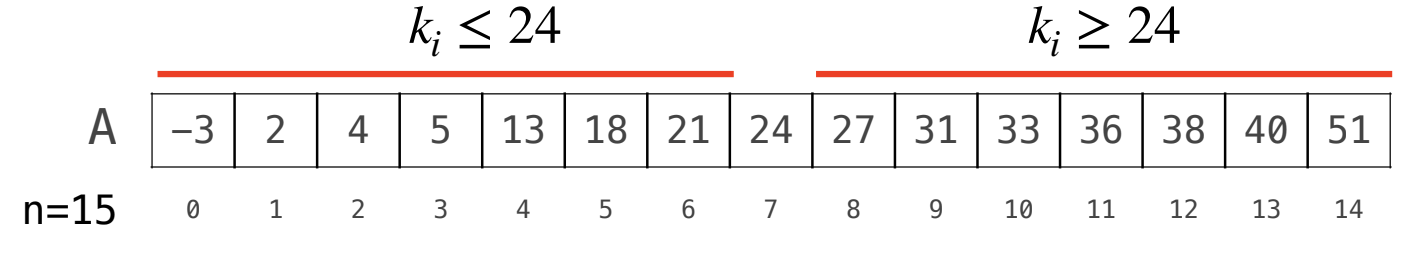
\includegraphics[width=9cm]{images/binary-search.png}
    \vspace{-8pt}
    \caption{Array A in BinarySearch}
    \label{fig:binary-search}
\end{figure}

\subsubsection{Codice dell'algoritmo}
\begin{lstlisting}[language=Javascript, caption=Codice BinarySearch]
function binSearch(k,A) {
    var pos:Int = -1;
    var sin:int = 0;
    var dx:Int = n - 1;
    while(sin <= dx && pos == -1){
        const cen:int = (sin + dx)/2;
        if (A[cen] == k) {pos = cen}
        else if (k < A[cen]) {dx = cen - 1}
        else {sin = cen + 1}
    }
    return pos;
}
\end{lstlisting}
Di seguito una spiegazione del funzionamento dell'algoritmo:
\begin{itemize}
    \item \textbf{Righe 2-4:} Andiamo ad inizializzare 3 variabili: "pos" che indicherà la posizione dell'elemento da cercare, viene inizializzata a -1 perché nel caso non si trovasse ritorna così -1. \\
    "Sin" che indica il capo sinistro della posizione che stiamo analizzando, e "dx" che indica il capo destro, sono entrambi inizialmente inizializzati come gli estremi dell'array.
    \item \textbf{Riga 5:} La condizione del while dice in sintesi che finché non abbiamo trovato il valore (pos == -1) e finchè "sin" e "dx" non si scambiano (che vorrebbe dire che abbiamo finito le iterazioni possibili), continuare a ciclare.
    \item \textbf{Righe 6-9:} All'interno del while quello che andiamo a fare e prendere il centro della porzione dell'array che stiamo considerando (inizialmente il centro dell'interno array) e vedere se il valore che dobbiamo cercare si trova in quella posizione, e in tal caso finiamo, è minore, e quindi si troverà alla sinistra del centro, o maggiore, in tal caso si troverà alla destra; nel caso non si sia trovato ci spostiamo ad analizzare la parte destra o sinistra asseconda del risultato. Eseguiamo questa operazioni finché è consentito dal ciclo.
\end{itemize}
\begin{note}
Nota che a noi non ci importa se la porzione è pari o dispari, quello che ci ritornerà esclude il resto.
\end{note}
\begin{example}
Esempio con l'array in figura \ref{fig:binary-search} cercando il valore 18.
\begin{table}[h!]
    \centering
    \setlength{\tabcolsep}{10pt}
    \renewcommand{\arraystretch}{1.8}
    \begin{tabular}{|c|c|c|c|c|}
    \hline
        pos & sin & dx & cen & A[cen]  \\\hline
        -1 & 0 & 14 & 7 & 24  \\\hline 
        -1 & 0 & 6 & 3 & 5  \\\hline
        -1 & 4 & 6 & 5 & \textbf{18}  \\
    \hline
    \end{tabular}
    \hspace{1cm}
    \begin{tabular}{|c|c|}
    \hline
        Iterazioni & Dimensione A \\\hline
        1 & n \: = \: n$/2^0$  \\\hline 
        2 & n/2 \: = \: n$/2^1$ \\\hline
        3 & n/4 \: = \: n$/2^2$ \\\hline
        ... & ... \\
    \hline
    \end{tabular}
    \caption{Esempio di funzionamento dell'algoritmo a sinistra e numero iterazione a destra}
\end{table}
\end{example}

\subsubsection{Calcolo caso pessimo e migliore}
Per calcolare il caso pessimo partiamo guardando la tabella sopra, notiamo che in questo algoritmo verranno eseguite $n/2^i$ operazioni, quindi il massimo possibile dipende da quanto è grande $i$. Per andare a trovare $i$ basta:
\begin{center}
    $n/2^i = 1$ \hspace{.3cm} $n = 2^i$ \hspace{.3cm} $\log_2n = \log_22^i$ \hspace{.3cm} $i = \log_2n \in O(\log_n)$
\end{center}
Questo caso è o quando k si trova agli estremi o quando k non c'è nell'array, e quindi ritorna -1.
\newpage
\section{Funzioni}
\begin{definition}[Funzione]
- $f: A \longrightarrow B$: \\
Dati due insiemi A, B, detti corrispettivamente dominio e codominio, una funzione è una "legge" o "regola" che associa ad ogni elemento di $a \in A$ uno ed uno solo elemento di B, che si denota con f(a).
\end{definition}
\begin{note}
Tipicamente in questo corso le funzioni saranno date come formule del tipo $f(x) = x^2 - 7x - e^x$ andando poi a specificare dominio e codominio in questo modo $f: \mathbb{R} \longrightarrow \mathbb{R}$
\end{note}
\begin{example}
    Esempi funzioni:
    \begin{itemize}
        \item $g(x) = x^2 - 7x - e^x$ \hspace{.3cm} $g(0,+\infty) \longrightarrow \mathbb{R}$
        \item $g(x) = x^2$ \hspace{.3cm} $g(0, +\infty) \longrightarrow (0, +\infty)$. \hspace{.3cm}Va bene perché $x^2 > 0$ per qualsiasi valore di x.
        \item $h(x) = x^2$ \hspace{.3cm} $h(0, +\infty) \longrightarrow (-\infty, 0)$. \hspace{.3cm}Questa forma non va bene non definendo una funzione perché la formula non mi da numeri di $(-\infty, 0)$.
        \item $h(x) = x^2$ \hspace{.3cm} $h(0, +\infty) \longrightarrow (-\infty,1)$ \hspace{.3cm}Non va bene perché se preindiamo x=3 $f(3) = 9$ e 9 non fa parte del codominio. 
    \end{itemize}
\end{example}
Una funzione $f: A \longrightarrow B$ con $A,B \in \mathbb{R}$ ha un \textbf{grafico} che si indica come:
\begin{equation}
    graph(f) = \{(a,b) \in A \:X\: B\ \:|\: b = f(a)\}
\end{equation}
\begin{wrapfigure}[8]{l}{7cm}
    \centering
    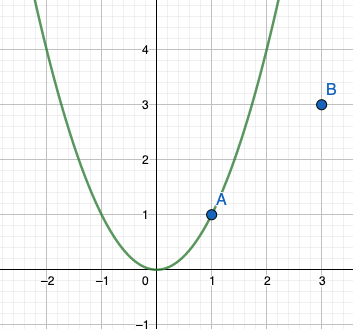
\includegraphics[width=4.5cm, height=4cm]{Esempio-grafico.png}
    \caption{$f(x) = x^2$ con $f: \mathbb{R} \longrightarrow \mathbb{R}$}
    \label{fig:esempio-grafico}
\end{wrapfigure}
\begin{example}
Esempio punto sulla funzione
\begin{itemize}
    \item Il punto A sta sul grafico si $f(x) = x^2$ esattamente quando $y = x^2$.
    \item Il punto B non sta sul grafico quindi $y \neq x^2$.
\end{itemize}
\end{example}
\begin{note}
    A X B $\subseteq \mathbb{R}$ X $\mathbb{R}$. Dove R X R = $R^2$.
\end{note}
\begin{example}
A e B = $(0, +\infty)$, da qui vediamo che A X B rappresenta il primo quadrante.\\\\
\end{example}

\subsection{Immagine}
\begin{definition}[Immagine]
Prendendo $f: A \longrightarrow B$ e $D \subseteq A$ l'immagine di D tramite f è il sottoinsieme $f(D) \subseteq B$ costituito dagli elementi f(d) dove $d \in D$.
\end{definition}
\begin{example}
    Esempi immagine:
    \begin{itemize}
        \item Immagine di A, $f(A) \subseteq B$ si chiama anche immagine della funzione.
        \item $f(x) = x^2$, $f: \mathbb{R} \longrightarrow \mathbb{R}$ \hspace{.2cm} immagine di g è $[0, +\infty)$ perché $x^2 \geq 0 \: \forall \: x \in \mathbb{R}$.
        \item $g(x) = x?2$, $g:[2, +\infty) \longrightarrow \mathbb{R}$ \hspace{.2cm} l'immagine di g è $[4, +\infty]$ perché se si calcola il punto minore del dominio, cioè 2, torna $g(2) = x^2$ che è uguale a 4, da lì possiamo prendere tutti i punti.
    \end{itemize}
\end{example}

\subsection{Suriettiva}
\begin{definition}[Suriettiva]
Una funzione si dice suriettiva quando ogni elemento del codominio è immagine di almeno un elemento del dominio. Quindi prendendo una f(x), per che sia suriettiva deve l'immagine I essere uguale ad un valore, $I(f) = b$.
\end{definition}
\begin{example}
    Esempi funzioni suriettive:
    \begin{itemize}
        \item $f(x) = x^2$, $f: \mathbb{R} \longrightarrow \mathbb{R}$ non è suriettiva perché tutti i valori del codominio $y < 0$ non hanno un rispettivo nel dominio.
        \item $g(x) = x^2$, $g: \mathbb{R} \longrightarrow (0, +\infty)$ lo è perchè andiamo a restringere il codominio ai punti che hanno un corrispettivo nel dominio.
    \end{itemize}
\end{example}

\subsection{Iniettiva}
\begin{definition}[Iniettiva]
Una funzione iniettiva è una funzione che associa, a elementi distinti del dominio, elementi distinti del codominio. Quindi prendendo una f(x) è iniettiva se prendendo due valori $x_1, x_2$ dove $x_1 \neq x_2 \Longrightarrow f(x_1) \neq f(x_2)$. (Input diversi danno output diversi).
\end{definition}
\begin{example}
    Esempi funzioni iniettiva:
    \begin{itemize}
        \item $f(x) = x^2$, $f: \mathbb{R} \longrightarrow \mathbb{R}$ non è iniettiva perché se prendiamo $x_1 = 1$ e $x_2 = -1$ $f(x1) = f(x2).$
        \item $g(x) = x^2$, $g: [0, +\infty) \longrightarrow \mathbb{R}$ è invece iniettiva perché non consideriamo i valori negativi.
    \end{itemize}
\end{example}

\subsection{Biunivoca}
\begin{definition}[Biunivoca]
Una funzione si definisce biunivoca o bigettiva se è sia iniettiva che suriettiva.
\end{definition}

\subsection{Invertibile}
\begin{definition}[Invertibile]
Se una funzione è biunivoca si dice che tale funzione è anche invertibile.
\end{definition}
\begin{wrapfigure}{l}{6cm}
    \centering
    \includegraphics[width=5cm, height=4cm]{Esempio-invertibilità.png}
    \caption{$f(x) = x^2$ e $g(x) = \sqrt{x}$}
    \label{fig:esempio-invertibilità}
\end{wrapfigure}
Se f è una funzione invertibile i grafici di f e di $f^i$ (la funzione inversa) sono simmetrici rispetto alla retta y=x cioè alla bisettrice del primo e del terzo quadrante. \\
\begin{example}
Se vediamo nell'immagine [\ref{fig:esempio-invertibilità}] prendendo l'inverso della funzione $f(x) = x^2$ definita in $[0, +\infty] \longrightarrow \mathbb{R}$ e cioè la funzione $g(x) = \sqrt{x}$ è simmetrica.
\\ \\ \\ \\ \\
\end{example}

\subsection{Funzioni Monotone}
\begin{definition}[Monotone]
Dato un insieme $A \in \mathbb{R}$ e $x_1, x_2 \in A$ con $x_1 < x_2$ se $\forall x_1, x_2$ risulta ciò che è scritto in Tabella \ref{tab:monotone}.
\end{definition}
\begin{table}[h!]
    \centering
    \setlength{\tabcolsep}{6pt}
    \renewcommand{\arraystretch}{1.7}
    \begin{tabular}{|c|c|}
        \hline
        \textbf{[1] Strettamente Crescente} & $f(x_1) < f(x_2) $ \\ \hline
        \textbf{[2]Debolmente Crescente} & $f(x_1) \leq f(x_2) $ \\ \hline
        \textbf{[3]Strettamente Decrescente} & $f(x_1) > f(x_2) $ \\ \hline
        \textbf{[4]Debolmente Decrescente} & $f(x_1) \geq f(x_2) $ \\ \hline
    \end{tabular}
    \caption{Definizioni funzioni crescenti e decrescenti}
    \label{tab:monotone}
\end{table}
Andando a considerare la Tabella \ref{tab:monotone} possiamo dire che:
\begin{itemize}
    \item \textbf{Strettamente monotona} nei casi [1] e [3] della tabella.
    \item \textbf{Debolmente monotona} nei casi [2] e [4] della tabella.
\end{itemize}

\begin{example}
    Esempi funzioni crescenti e decrescenti:\\
    \begin{figure}[h!]
        \begin{subfigure}{.5\textwidth}
            \centering
            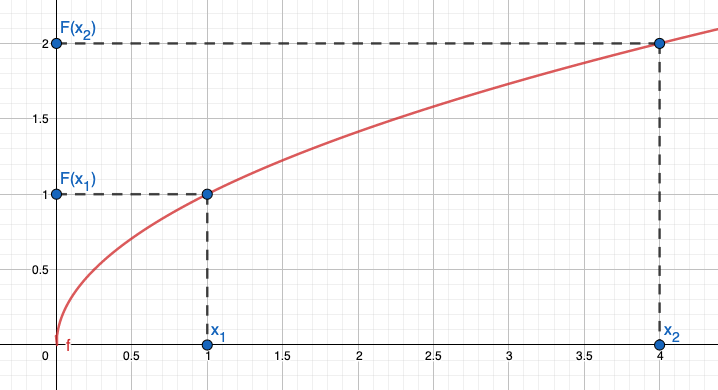
\includegraphics[width=6cm, height=4cm]{funzione-crescente.png}
            \caption{$f(x_1) < f(x-2)$ quindi è crescente}
            \label{fig:funzione-crescente}
        \end{subfigure}
        \begin{subfigure}{.5\textwidth}
            \centering
            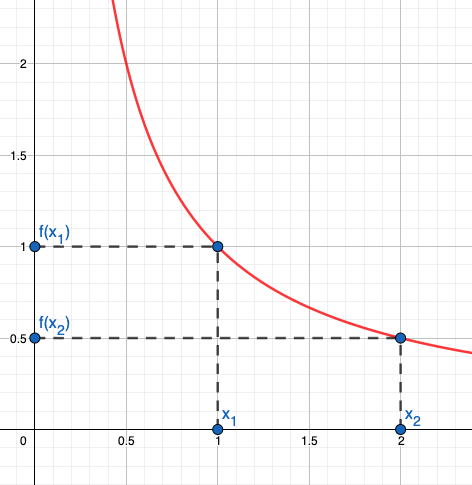
\includegraphics[width=6cm, height=4cm]{funzione-decrescente.png}
            \caption{$f(x_1) > f(x-2)$ quindi è decrescente}
            \label{fig:funzione-decrescente}
        \end{subfigure}
    \end{figure}
    \\Possiamo anche federe dalle immagini [\ref{fig:funzione-crescente}] [\ref{fig:funzione-decrescente}] che:
    \begin{itemize}
        \item Se f(x) è \textbf{crescente} l'ordinamene verrà \textbf{mantenuto}.
        \item Se f(x) è \textbf{decrescente} l'ordinamento verrà \textbf{invertito}.\\
    \end{itemize}
\end{example}

\begin{observation}
    Osservazione sul rapporto incrementale:\\
\end{observation}
\begin{wrapfigure}[8]{l}{8cm}
    \vspace{-15pt}
    \centering
    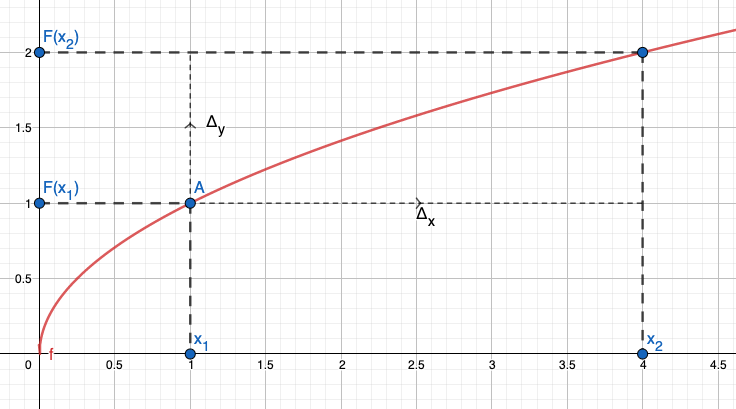
\includegraphics[width=6.7cm]{rapporto_incrementale.png}
    \caption{$\frac{\Delta_y}{\Delta_x}$}
    \label{fig:esempio-invertibilità}
\end{wrapfigure}
f(x) è strettamente crescente se e solo se il \textbf{rapporto incrementale}\footnote{I rapporto incrementale misura quanto il punto della f si sposta in verticale in rapporto a quanto abbiamo l'asciasse in orizzontale.} è maggiore di 0:
\begin{equation}
    \frac{f(x_1) - f(x_2)}{x_1 - x_2} > 0
\end{equation}
\begin{note}
    Il denominatore ed il numeratori devono essere concordi per fare in modo che il rapporto incrementale sia maggiore di 0 e quindi la funzione crescente. \\ \\\\
\end{note}
Continuando ad analizzare il rapporto incrementale possiamo ricavare anche i casi in cui una funzione e strettamente decrescente o debolmente crescente o debolmente decrescente. Puoi vedere tutte le casistiche nella tabella \ref{tab:analisi-rapporto-incrementale}.
\begin{table}[h!]
    \centering
    \setlength{\tabcolsep}{7pt}
    \renewcommand{\arraystretch}{2}
    \begin{tabular}{|c|c|}
        \hline
        Strettamente Crescente & $\frac{f(x_1) - f(x_2)}{x_1 - x_2} > 0$\\ \hline
        Strettamente Decrescente & $\frac{f(x_1) - f(x_2)}{x_1 - x_2} < 0$ \\ \hline
        Debolmente Crescente & $\frac{f(x_1) - f(x_2)}{x_1 - x_2} \geq 0$ \\ \hline
        Debolmente Decrescente & $\frac{f(x_1) - f(x_2)}{x_1 - x_2} \leq 0$ \\ \hline
    \end{tabular}
    \caption{Analisi rapporto incrementale}
    \label{tab:analisi-rapporto-incrementale}
\end{table}
\begin{observation}
    Se una funzione f(x) è strettamente crescente è a sua volta anche debolmente crescente, mentre una funzione f(x) se è debolmente crescente non è strettamente crescente perché aggiunge una casistica che sarebbe $f(x_1) = f(x_2)$. 
\end{observation}
\begin{example}
    Casistica particolare:\\
    Data $f(x)=\frac{1}{x}$, \hspace{.3cm} $f: \mathbb{R} \: \setminus \: \{0\} \longrightarrow \mathbb{R} \: \setminus \: \{0\}$. Funzione rappresentata nell'immagine [\ref{fig:esempio-particolare}].
    \begin{figure}[h!]
        \centering
        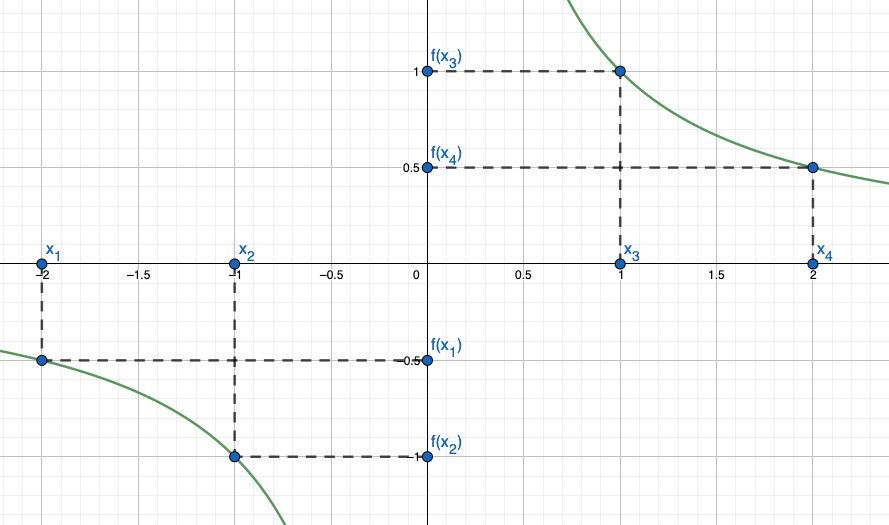
\includegraphics[width=8.7cm]{esempio-particolare.png}
        \caption{$f(x)=\frac{1}{x}$, \hspace{.3cm} $f: \mathbb{R} \: \setminus \: \{0\} \longrightarrow \mathbb{R} \: \setminus \: \{0\}$}
        \label{fig:esempio-particolare}
    \end{figure}
    \\Possiamo vedere che:
    \begin{itemize}
        \item f(x) è strettamente decrescente in $(0, +\infty)$.\\
        Quindi se andiamo a prendere $0 < x_3 < x_4$ abbiamo che $f(x_3) > f(x_4)$.
        \item f(x) è strettamente decrescente in $(-\infty, 0)$.\\
        Quindi se andiamo a prendere $x_1 < x_2 < 0$ abbiamo che $f(x_1) > f(x_2)$.
    \end{itemize}
    Se però andiamo a considerare tutto $\mathbb{R} \: \setminus \: \{0\}$, e quindi prendiamo i punti $x_1 < 0 < x_4$ vediamo che $f(x_1) < f(x_4)$.
    In conclusione si può dire quindi che $f(x)=\frac{1}{x}$) è decrescente in $(-\infty, 0)$ e in $(0, +\infty)$ ma non lo è in tutto $\mathbb{R} \: \setminus \: \{0\}$.
\end{example}

\subsubsection{Composizione con funzioni monotone}
\begin{note}
     Il simbolo della composizione è "$\circ$", come $f \circ g$.
\end{note}
Prendendo i considerazioni 3 insiemi A, B, C tali che $A, B, C \subset \mathbb{R}$ e 2 funzioni f(x) e g(x) così definitine: \hspace{.2cm} $f: A \longrightarrow B$, $g: B \longrightarrow C $.
\begin{enumerate}
    \item Se f è crescente e g è crescente allora $g \circ f$ è crescente.
    \item Se f è crescente e g è decrescente allora $g \circ f$ è decrescente. (Vale anche l'inverso).
    \item Se f è decrescente e g è decrescente allo $g \circ f$ è crescente. 
\end{enumerate}
\begin{example}
    $h(x) = e^{x^3}$\\
    La funzione h si ottiene dalla composizione di:
    \begin{itemize}
        \item $f: \mathbb{R} \longrightarrow \mathbb{R}$ \hspace{.3cm} $f(x) = x^3$. Funzione crescente.
        \item $g: \mathbb{R} \longrightarrow \mathbb{R}$ \hspace{.3cm} $g(t) = e^t$. Funzione decrescente.
    \end{itemize}
    Quindi possiamo scrivere $h(x) = e^{x^3}$ come: \hspace{.3cm} $e^{f(x)} \: \: = \: \: g(f(x)) \: \: = \: \: (g \circ f)(x)$
    Inoltre visto che f è crescente e g è crescente, h è strettamente crescente 
\end{example}
\begin{observation}
    Se prendiamo una funzione f(x) strettamente monotona, allora f(x) è iniettiva. Questa condizione è vera ma NON lo è viceversa: una funzione f(x) iniettiva NON è per forza strettamente monotona. 
\end{observation}
\begin{example}
    Se prendiamo una f(x) tale che: \hspace{.3cm} $f(x) = \frac{1}{x}$ \hspace{.3cm} $\mathbb{R} \setminus \{0\} \longrightarrow \mathbb{R} \setminus \{0\}$
    \\Possiamo vedere rifacendoci all'esempio in figura [\ref{fig:esempio-particolare}] che f è iniettiva ma non monotona.
\end{example}

\subsection{Insieme di definizione}
\begin{definition}[Insieme di definizione]
    Prendendo una funzione f(x) l'insieme di definizione o dominio naturale di una funzione è il più grande sottoinsieme di $\mathbb{R}$ dove ha senso la funzione f(x).
\end{definition}
\begin{example}
    $f(x) = \frac{1}{x}$ \hspace{.3cm} L'insieme di definizione è $\mathbb{R} \setminus \{0\}$
\end{example}

\subsection{Funzioni pari e dispari}
\begin{definition}[Pari]
    La funzione è \textbf{Pari} se $f(x) = f(-x) \: \forall x$ nel dominio di $f \longrightarrow f$.
\end{definition}
\begin{definition}[Dispari]
    La funzione è \textbf{Dispari} se $f(x) = -f(-x) \: \forall x$ nel dominio di $f \longrightarrow f$.
\end{definition}
\begin{note}
    Il dominio di f deve essere tale che se $x \in Dominio$ allora $-x \in Codominio$.\\
\end{note}
\begin{example}
Esempio funzioni pari e dispari.\\
\end{example}
$f(-x) = (-x)^2 = x^2 = f(x)$, f(x) è \textbf{pari}: \hfill $f(-x) = (-x)^2 = x^2 = -f(x)$, f(x) è \textbf{dispari}:
\begin{figure}[h!]
    \vspace{-1pt}
    \begin{subfigure}{.5\textwidth}
        \centering
        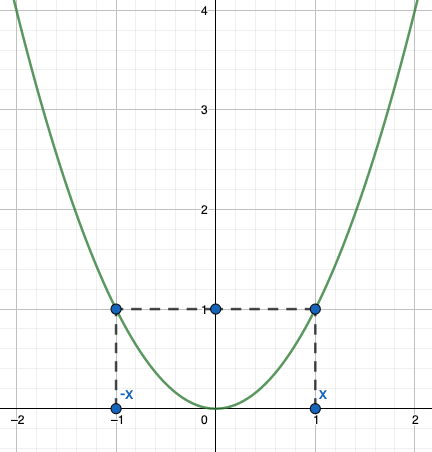
\includegraphics[width=3cm]{funzione-pari.png}
        \caption{$f(x) = x^2$, \hspace{.2cm} graph(f) con f pari}
    \end{subfigure}
    \begin{subfigure}{.5\textwidth}
        \centering
        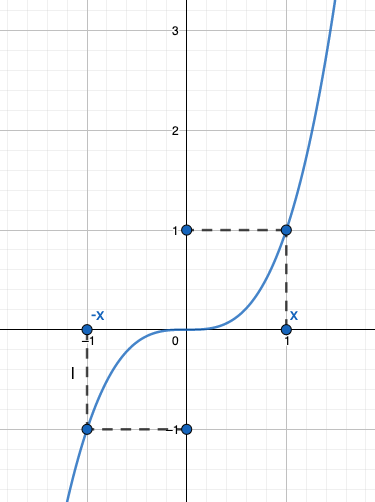
\includegraphics[width=2.5cm]{funzione-dispari.png}
        \caption{$f(x) = x^3$, \hspace{.2cm} graph(f) con f dispari}
    \end{subfigure}
\end{figure}

\subsection{Funzione periodica}
\begin{definition}[Periodicità]
    Una funzione f(x) si dice periodica di periodo $P \in \mathbb{R}$ se $\forall x \: \: f(x + P) = f(x)$. 
\end{definition}
\begin{wrapfigure}{r}{9cm}
    \vspace{-15pt}
    \centering
    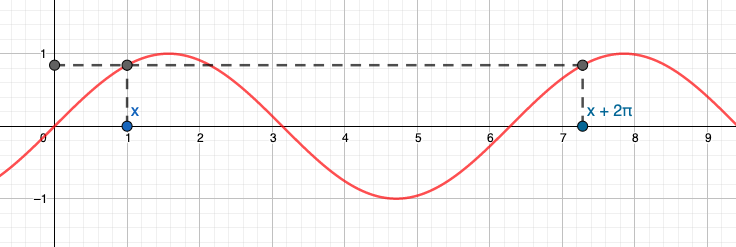
\includegraphics[width=7cm]{funzione-periodica.png}
    \caption{$sin(x) = sin(x + 2\pi)$}
    \label{fig:funzione-periodica}
\end{wrapfigure}
Inoltre il dominio di f(x) deve essere tale che $x \in$ Dominio è uguale e a $x + P \in$ codominio.
\begin{example}
In figura [\ref{fig:funzione-periodica}] un esempio di funzione periodica.\\\\
\end{example}

\newpage
\subsection{Funzioni Elementari}
\subsubsection{Retta}
\textbf{Funzione retta:} $f(x) = ax + b$. \hspace{.3cm} $a,b \in \mathbb{R}$ \\ Dove la "a" si dice coefficiente angolare, ed indica la pendenza della retta mentre la lettera "b" si chiama termine noto, ed indica il punto di incontro con l'asse Y.

\subsubsection{Esponente positivo o negativo}
\textbf{Fun. Esp. positivo:} $f(x) = x^k$, $k \in \mathbb{N}$. \hfill \textbf{Fun. Esp. negativo:} $f(x) = x^k$, $k \in \mathbb{N}$, $k < 0$.
\begin{figure}[h!]
    \begin{subfigure}{.5\textwidth}
        \centering
        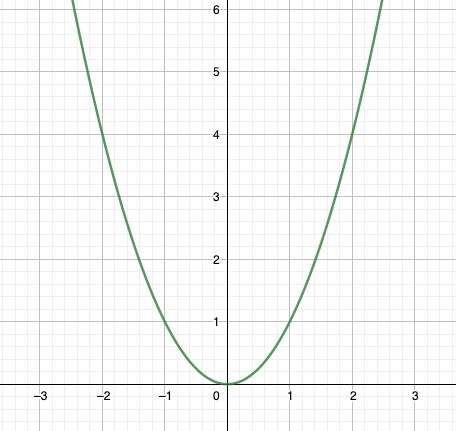
\includegraphics[width=4cm, height=3.5cm]{parabole.png}
        \caption{con k pari}
        \label{fig:esponente-positivo-pari}
    \end{subfigure}
    \begin{subfigure}{.5\textwidth}
        \centering
        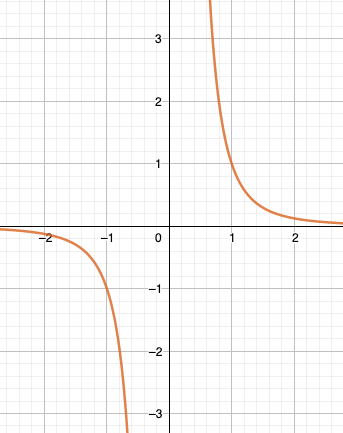
\includegraphics[width=4cm, height=3.5cm]{esponente-negativo-dispari.png}
        \caption{con k dispari}
        \label{fig:esponente-positivo-dispari}
    \end{subfigure}
\end{figure}
\begin{figure}[h!]
    \vspace{-5pt}
    \begin{subfigure}{.5\textwidth}
        \centering
        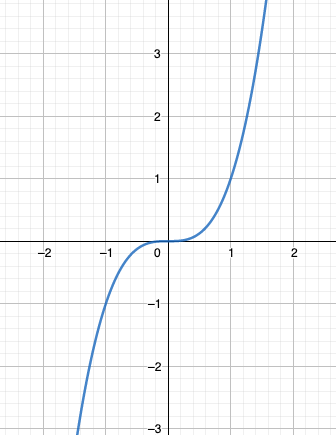
\includegraphics[width=4cm, height=3.7cm]{esponente-dispari.png}
        \caption{con k pari}
        \label{fig:esponente-negativo-pari}
    \end{subfigure}
    \begin{subfigure}{.5\textwidth}
        \centering
        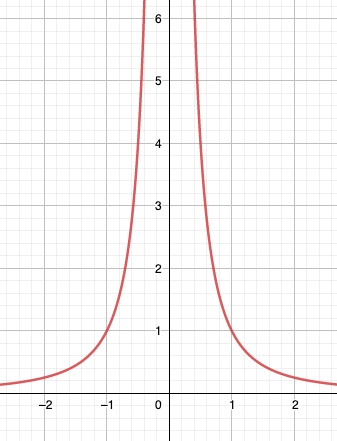
\includegraphics[width=4cm, height=3.5cm]{esponsente-negativo-pari.png}
        \caption{con k dispari}
        \label{fig:esponente-negativo-dispari}
    \end{subfigure}
\end{figure}
\begin{observation}
    \textbf{k pari:} Le funzioni con il k pari sono funzioni pari e hanno tutte una forma simile a quella in figura [\ref{fig:esponente-positivo-pari}] per le funzioni con k positive e per le funzioni con k negativo figura [\ref{fig:esponente-negativo-pari}].
\end{observation}
\begin{observation}
    \textbf{k dispari:} Le funzioni con il k positivo e dispari sono funzioni dispari e hanno tutte una forma simile a quella in figura [\ref{fig:esponente-positivo-dispari}] per le funzioni con k positive e per le funzioni con k negativo figura [\ref{fig:esponente-negativo-dispari}].
\end{observation}

\subsubsection{Radici o esponente fratto}
\textbf{Funzionane radici o esponente fratto:} $f(x) = x^{\frac{p}{q}}$ o $f(x) = \sqrt[q]{x^p}$  \: \: con  \: \:  $p, q \in \mathbb{N}$ \: \: e  \: \:  $q \neq 0$. \footnote{In matematica è possibile scrivere una un esponente fratto come radice mettendo il numeratore al radicando della radice e il denominatore all'indice: $x^{\frac{p}{q}} \: = \: \sqrt[q]{x^p}$}
\begin{figure}[h!]
    \begin{subfigure}{.5\textwidth}
        \centering
        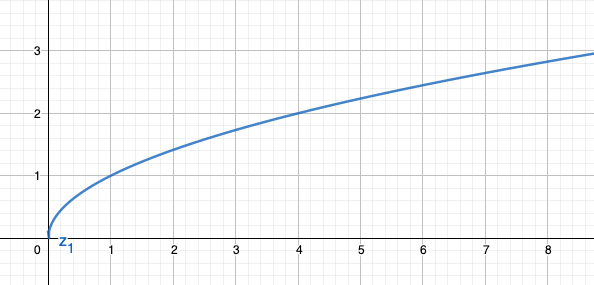
\includegraphics[width=6.3cm]{radice-pari.png}
        \caption{con q pari}
        \label{fig:radice-pari}
    \end{subfigure}
    \begin{subfigure}{.5\textwidth}
        \centering
        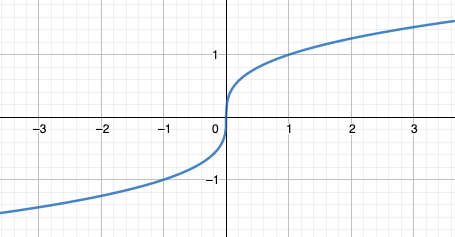
\includegraphics[width=6cm]{radice-dispari.png}
        \caption{con q dispari}
        \label{fig:radice-dispari}
    \end{subfigure}
\end{figure}
\begin{note}
    p e q non possono essere entrambi pari perché in tal caso sono divisibili fra di loro e quindi portabili ad una forma ridotta.
\end{note}
\begin{observation}
    \textbf{q pari:} Le funzioni con il q pari ha dominio $ x \geq 0$ ed è invertibile sono come funzione $f: [0, +\infty) \longrightarrow [0, +\infty)$. È rappresentata in figura [\ref{fig:radice-pari}].
\end{observation}
\begin{observation}
    \textbf{q dispari:} Le funzioni con il q positivo ha dominio $x \in \mathbb{R}$ ed è ugualmente invertibile su tutto $\mathbb{R}$, è inoltre una funzione dispari. È rappresentata in figura [\ref{fig:radice-dispari}].\\
\end{observation}

\subsubsection{Esponenziale}
\textbf{Funzione esponenziale:} $f(x) = a^x$ con $a \in \mathbb{R}$, \: \: $a > 0$, \: \: $a \neq 1$ \: \: $f: \mathbb{R} \longrightarrow (0, +\infty)$
\begin{figure}[h!]
    \begin{subfigure}{.5\textwidth}
        \centering
        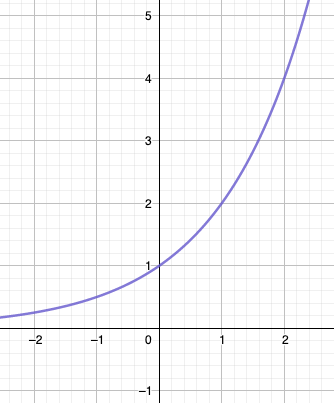
\includegraphics[width=4cm]{esponenziale.png}
        \caption{con $a > 1$}
        \label{fig:esponenziale}
    \end{subfigure}
    \begin{subfigure}{.5\textwidth}
        \centering
        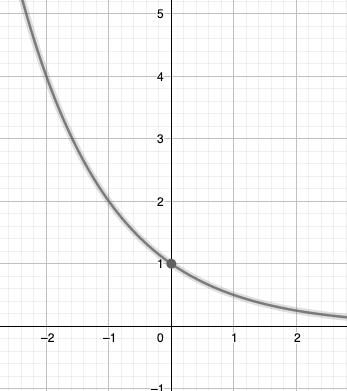
\includegraphics[width=4cm]{esponsenziale-base-minore.png}
        \caption{con $0 < a < 1$}
        \label{fig:esponsenziale-base-minore}
    \end{subfigure}
\end{figure}
\begin{note}
    La funzione esponenziale è sempre positiva.
\end{note}
\begin{observation}
    \textbf{$a > 1$:} La funzione è strettamente crescente, come in nell'immagine [\ref{fig:esponenziale}].
\end{observation}
\begin{observation}
    \textbf{$0 < a < 1$:} La funzione è decrescente, come in nell'immagine [\ref{fig:esponsenziale-base-minore}].
\end{observation}

\subsubsection{Logaritmo}
\textbf{Funzione logaritmo:} $f(x) = \log_a x$, \: \: $f: (0, +\infty) \longrightarrow \mathbb{R}$ \: \: (inversa dell'esponenziale).
\begin{figure}[h!]
    \begin{subfigure}{.5\textwidth}
        \centering
        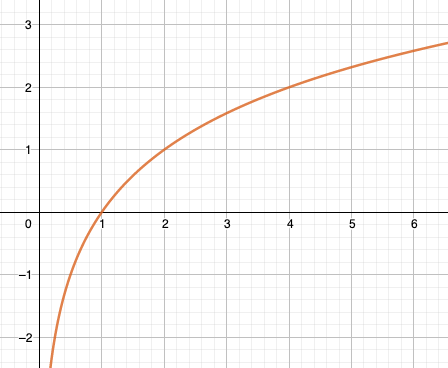
\includegraphics[width=5cm,height=4cm]{logaritmo.png}
        \caption{con $a > 1$}
        \label{fig:logaritmo}
    \end{subfigure}
    \begin{subfigure}{.5\textwidth}
        \centering
        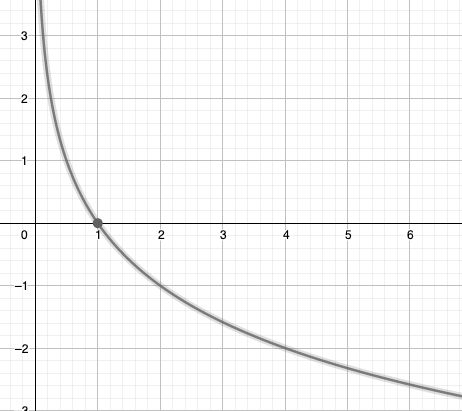
\includegraphics[width=5cm,height=4cm]{logaritmo-base-minore.png}
        \caption{con $0 < a < 1$}
        \label{fig:logaritmo-base-minore}
    \end{subfigure}
\end{figure}
\begin{observation}
    Casistica particolare - $f(x) = e^x$.\\
    In questa casistica se andiamo a ridurre il codominio la funzione esponenziale è invertibile. $f: \mathbb{R} \longrightarrow (0, +\infty)$.
    Il suo inverso è un caso particolare di logaritmo e di chiama \textbf{logaritmo naturale}. E si può scrive in due modi:
    \begin{itemize}
        \item $\ln{x}$: sarebbe logaritmo in base naturale.
        \item $\log x$: scrivendo il logaritmo senza la base intendiamo il logaritmo in base $e$.
    \end{itemize}
\end{observation}

\subsubsection{Seno e Arcoseno}
\textbf{Seno:} $f(x) = \sin x$, $f: \mathbb{R} \longrightarrow \mathbb{R}$. \hfill
\textbf{Arcoseno:} $f(x) = \arcsin x$, $f: [-1, 1] \longrightarrow [-\frac{\pi}{2}, \frac{\pi}{2}]$
\begin{figure}[h!]
    \begin{subfigure}{.5\textwidth}
        \centering
        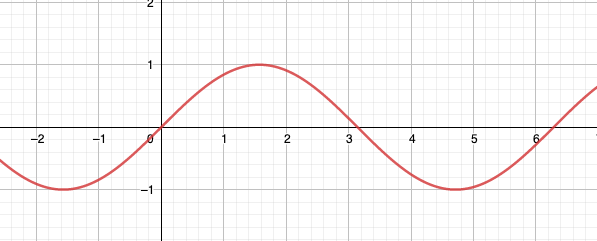
\includegraphics[width=6cm]{seno.png}
        \caption{$\sin{x}$}
        \label{fig:seno}
    \end{subfigure}
    \begin{subfigure}{.5\textwidth}
        \centering
        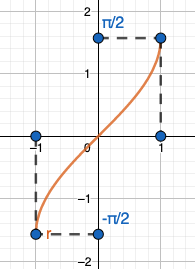
\includegraphics[width=2cm, height=2.3cm]{arcoseno.png}
        \caption{$\arcsin{x}$ o $\sin{x}^{-1}$}
        \label{fig:arcoseno}
    \end{subfigure}
\end{figure}

\begin{observation}
    \textbf{Sin(x):} La funzione $\sin{x}$ (immagine [\ref{fig:seno}]) è periodica per $2\pi$ quindi possiamo scrivere $\sin{(x+2\pi)} = \sin x \: \forall x \in \mathbb{R}$. Inoltre è suriettiva per codominio [-1, 1]. Se invece definiamo $f: [-\frac{\pi}{2}, \frac{\pi}{2}] \longrightarrow [-1, 1]$ la funzione $\sin x$ è strettamente crescente e suriettiva, quindi anche invertibile, e la sua inversa è appunto $\arcsin{x}$.
\end{observation}
\begin{observation}
    \textbf{Arcsin(x):} La funzione $\arcsin{x}$ è l'inverso del seno e può essere scritta anche come $f(x) = \sin{x}^{-1}$, è rappresentata nell'immagine [\ref{fig:arcoseno}].
\end{observation}

\subsubsection{Coseno e Arcocoseno}
\textbf{Coseno:} $f(x) = \cos{x}$, $f: \mathbb{R} \longrightarrow \mathbb{R}$. \hfill
\textbf{Arcocoseno:} $f(x) =\arccos{x}$, $f: [-1, 1] \longrightarrow [0, \pi]$
\begin{figure}[h!]
    \begin{subfigure}{.5\textwidth}
        \centering
        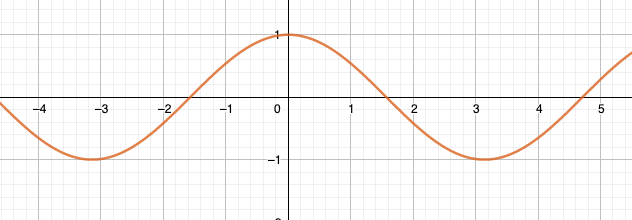
\includegraphics[width=6cm]{coseno.png}
        \caption{$\cos{x}$}
        \label{fig:coseno}
    \end{subfigure}
    \begin{subfigure}{.5\textwidth}
        \centering
        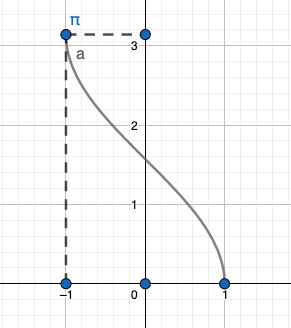
\includegraphics[width=3.5cm, height=2.7cm]{arcocoseno.png}
        \caption{$\arccos{x}$ o $\cos{x}^{-1}$}
        \label{fig:arcocoseno}
    \end{subfigure}
\end{figure}
\vspace{-5pt}
\begin{observation}
    \textbf{Cos(x):} La funzione $\cos{x}$, rappresentata nell'immagine [\ref{fig:coseno}], è periodica per $2\pi$ quindi possiamo scrivere $\cos{(x+2\pi)} = \cos x \: \forall x \in \mathbb{R}$. Inoltre è suriettiva per codominio [-1, 1]. Se invece definiamo $f: [0, \pi] \longrightarrow [-1, 1]$ la funzione $\cos x$ è suriettiva, quindi anche invertibile, e la sua inversa è appunto $\arccos{x}$.
\end{observation}
\begin{observation}
    \textbf{Arccos(x):} La funzione $\arccos{x}$ è l'inverso del seno e può essere scritta anche come $f(x) = \cos{x}^{-1}$ ed è rappresentata nell'immagine [\ref{fig:arcocoseno}].
\end{observation}

\subsubsection{Tangente e Arcotangente}
\textbf{Tangente:} $f(x) = \tan{x}$, $f: \mathbb{R} \longrightarrow \mathbb{R}$ \hfill
\textbf{Arcotangente:} $f(x) = \arctan{x}$, $f: \mathbb{R} \longrightarrow [-\frac{\pi}{2}, \frac{\pi}{2}]$
\begin{figure}[h!]
    \begin{subfigure}{.5\textwidth}
        \vspace{-20pt}
        \centering
        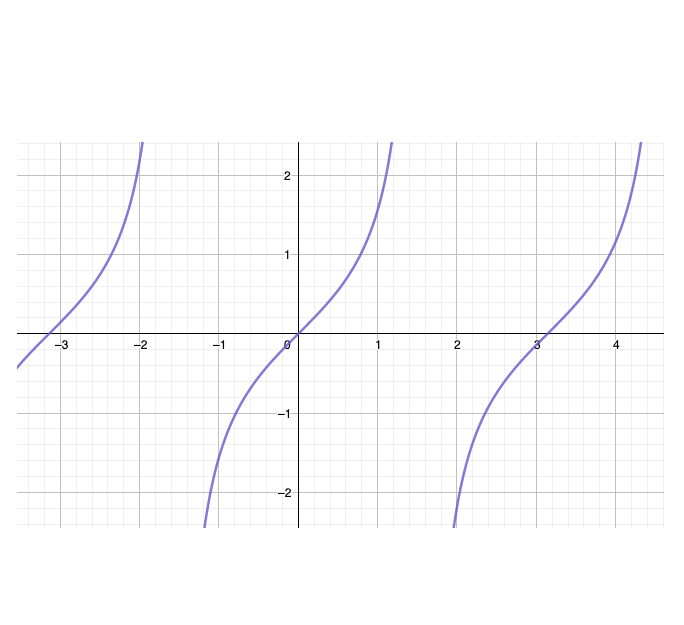
\includegraphics[width=4.2cm]{tangente.png}
        \vspace{-20pt}
        \caption{$\tan{x}$}
        \label{fig:tangente}
    \end{subfigure}
    \begin{subfigure}{.5\textwidth}
        \centering
        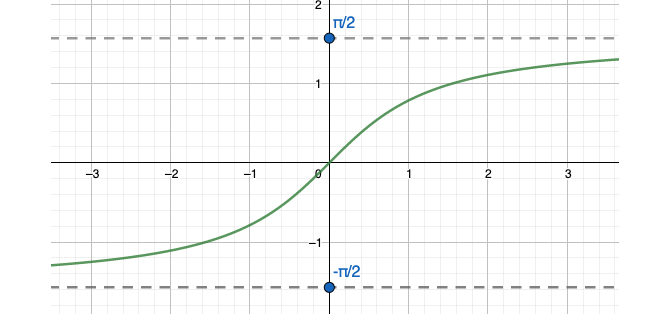
\includegraphics[width=5cm]{arcotangente.png}
        \caption{$\arctan{x}$ o $\tan{x}^{-1}$}
        \label{fig:arcotangente}
    \end{subfigure}
\end{figure}
\begin{observation}
    \textbf{Tan(x):} La funzione $\tan{x}$, rappresentata nell'immagine [\ref{fig:tangente}], può essere scritta anche come $\frac{\sin{x}}{\cos{x}}$, ha come dominio $\{x \in \mathbb{R} \: | \:  x \neq \frac{\pi}{2} + k\pi, \: k \in \mathbb{Z}\}$. La funzione tangente è fatta da infiniti intervalli, è quindi periodica per $\pi$; è di base non invertibile, ma se la ristringiamo in $f: [-\frac{\pi}{2}, \frac{\pi}{2}] \longrightarrow \mathbb{R}$ diventa biunivoca ed accetta la funzione inversa che è $\arctan{x}$.
\end{observation}
\begin{observation}
    \textbf{Arctan(x):} La funzione $\arctan{x}$, rappresentate nell'immagine [\ref{fig:arcotangente}], è inversa della funzione $\tan{x}$, può quindi essere scritta anche con la forma $\tan{x}^{-1}$.
\end{observation}
\newpage
\section{Gestione della memoria}
\subsection{Record di attivazione}
\begin{definition}
	è l'insieme di strutture dati e funzioni necessarie all'esecuzione dei programmi viene aggiunto al codice eseguibile dal compilatore.
\end{definition}
\begin{definition}[Activation record o stack frame]
	Contiene tutte le informazioni necessarie all'esecuzione del blocco o della funzione.
\end{definition}
\begin{definition}[Dynamic chain o call chain]
	Rappresenta la sequenza di chiamate e e serve a garantire il corretto ordine di esecuzione.
\end{definition}
\begin{definition}[Static chain]
	Implementa lo scoping statico e garantisce che i nomi siano referenziati rispettando la visibilità di variabili e funzioni.
\end{definition}
\begin{tabular} { |c|p{250px}|}
	\hline
	Puntatore catena dinamica  & Indirizzo del record di attivazione della funzione chiamante\\
	\hline
	Puntatore catena statica & Indirizzo del prossimo record di attivazione dove risolvere i nomi
		non presenti nel blocco corrente (implementazione dello scoping
		statico) \\
	\hline
	Indirizzo di ritorno & Indirizzo dell’istruzione da eseguire al termine della funzione/blocco corrente \\
	\hline
	Indirizzo risultato & Indirizzo nel record di attivazione del chiamante per memorizzare il risultato \\
	\hline
	Parametri & Spazio riservato alla associazione parametri formali - parametri attuali \\
	\hline
	Variabili locali & Spazio riservato alla allocazione delle variabili locali al blocco \\
	\hline
	Risultati temporanei & Spazio riservato alla allocazione delle variabili temporanee generate dal compilatore \\
	\hline
\end{tabular}
\subsection{Divisione della memoria}
\begin{figure}[h!]
	\centering
	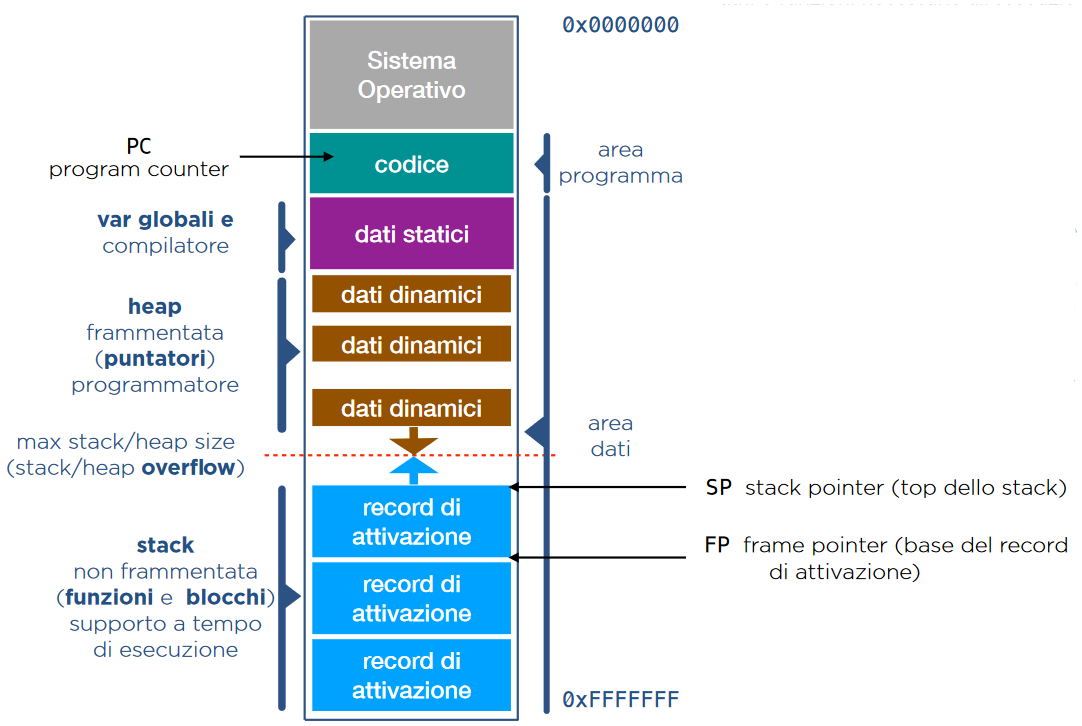
\includegraphics[width=13cm]{images/gestione-memoria.png}
	\caption{Gestione della memoria di un programma}
\end{figure}
\begin{note}
	Partiamo dal presupposto che un \textbf{blocco} sia considerato come una funzione senza parametri.
\end{note}
\newpage
\section{Ricorsione}
\begin{definition}[Ricorsione]
	A tempo di \textbf{compilazione}: una funzione usa il suo nome (chiama se stessa) nel suo corpo.
	A tempo di \textbf{esecuzione}: chiamate annidate della \textbf{stessa} funzione
\end{definition}
\noindent Una funzione ricorsiva è chiamata per risolvere un problema scomposto in:
\begin{itemize}
	\item \textbf{Caso base}: la funzione restituisce un valore
	\item \textbf{Passo ricorsivo}: la funzione viene chiamata su un problema analogo a quello iniziale ma di dimensioni minori, avvicinandosi al \emph{caso base}
\end{itemize}
Quando si  arriva al caso base viene effettuata una sequenza inversa di return statement, combinando i risultati parziali in quello finale.
\begin{example}[Fattoriale]
	Il fattoriale di un intero non negativo n è il prodotto
	degli interi positivi $<= n$ escluso lo $0$. Si indica con
	$n!$ e si impone per definizione $0! = 1$.
	\begin{equation}
		n! = \prod_{i=1}^{n} i=n*(n-1)*\ldots*1
	\end{equation}
	oppure definita in maniera ricorsiva:
	\begin{equation}
		n! = \begin{cases}
			1, \hspace{50px} n=0 \\
			n*(n-1)!, \hspace{6px} n>0
		\end{cases}
	\end{equation}
	In maniera programmatica possiamo scriverlo come:
	\begin{lstlisting}[language=Swift, caption=Fattoriale con ricorsione, mathescape=true]
		func F(var n: Int) -> Int {
			if (n-1) {
				return 1
			} else {
				return n * F(n-1)
			}
		}
	\end{lstlisting}
\end{example}

\subsection{Ricorsione e iterazione}
\begin{tabular} { |c|p{150px}|p{150px}|}
	\hline
	& \textbf{Ricorsione} & \textbf{Iterazione} \\
	\hline
	Controllo di terminazione & Condizione di ricorsione & Condizione di controllo nel loop \\
	\hline
	Ripetizioni & Chiamate ricorsive della funzione & Esecuzione ripetuta del corpo dell'iterazione \\
	\hline
	Convergenza alla terminazione & I passi ricorsivi riducono il problema al caso base & Il contatore si avvicina al valore di termine \\
	\hline
	Ripetizione infinita & Il passo ricorsivo non riduce il problema e non si avvicina al caso base & La condizione di controllo non è mai falsa \\
	\hline
\end{tabular}
\vspace{15pt}

\noindent Nella \emph{ricorsione}, al contrario dell'\emph{iterazione}, ogni chiamata alla funzione genera un nuovo record di attivazione contenente una nuova copia delle variabili e consumando lo stack di esecuzione. Questo può generare \textbf{overhead}.\\
In generale ogni problema \emph{ricorsivo} può essere anche scritto \emph{iterativamente}. È consigliato scriverlo ricorsivamente quando ciò facilita la lettura del problema stesso.
\newpage
\section{Condizioni}
\subsection{Condizioni su array}
Dato un array \textbf{a} di dimensione N, voglio verificare se la proprietà P vale per tutti gli elementi dell'array.
\begin{equation}
	\forall i \in [0, N).\mathcal{P}(a[i])
\end{equation}
\begin{example}
	Verifico che tutti gli elementi dell'array siano dispari.
	\begin{equation}
		\forall i \in [0, N).a[i]%2==1
	\end{equation}
	\begin{lstlisting}[language=C, caption=Verifica di proprietà su tutti gli elementi mathescape=true]
		int check_array_dispari(int a[], size_t dim) {
			int indice = 0;
			while (indice < dim && a[indice]%2 == 1){
				indice++;
			}
			if (indice == dim) {
				return 1;
			} else {
				return 0;
			}	
		}
	\end{lstlisting}
	Blocco lo scorrimento dell'array quando la proprietà \textbf{NON} viene soddisfatta almeno una volta.
\end{example}

\noindent
Se invece voglio verificare che la proprietà P valga per almeno un elemento:
\begin{equation}
	\exists i \in [0, N).\mathcal{P}(a[i])
\end{equation}
\begin{example}
	Verifico che almeno un elemento dell'array è uguale a 26.
	\begin{equation}
		\exists i \in [0, N).a[i]==26
	\end{equation}
	\begin{lstlisting}[language=C, caption=Verifica di proprietà su almeno un elemento, mathescape=true]
		int esiste_in_array(int a[], size_t dim, in n) {
			size_t indice = 0;
			_Bool trovato = 0;
			while (indice < dim && !trovato){
				if(a[indice] == n) {
					trovato = 1;	
				}
				indice++;
			}
			return trovato;
		}
	\end{lstlisting}
	Blocco lo scorrimento dell'array nel momento in cui trovo un elemento che soddisfa la proprietà, utilizzando un \textit{flag}.
\end{example}
\subsection{Condizioni su matrici}
Una \textbf{matrice} è un array di array. Può essere \textit{multidimensionale} $N \times M$ e voglio verificare se tutti i suoi elementi oppure solo uno di essi verificano una proprietà P.
\begin{equation}
	\forall i \in [0, N), \forall j \in [0,M).\mathcal{P}(a[i,j])
\end{equation}
\begin{equation}
	\exists i \in [0, N), \exists j \in [0,M).\mathcal{P}(a[i,j])
\end{equation}
\begin{definition}[Matrice quadrata]
	Una matrice è \textbf{quadrata} se a lo stesso numero di righe e di colonne. In questo caso per scorrerla si può usare un solo indice:
	\begin{equation}
		\exists i,j \in [0, N).\mathcal{P}(a[i,j])
	\end{equation}
\end{definition}

\begin{example}
	Verifico se tutti gli elementi della matrice sono positivi.
	\begin{equation}
		\forall i \in [0, N), \forall j \in [0, M) . a[i, j] > 0
	\end{equation}
	\begin{lstlisting}[language=C, caption=Verifica di proprietà su tutti gli elementi della matrice, mathescape=true]
		int check_matrice_pos(int a[][COL], size_t dim) {
			size_t row, col;
			row = col = 0;
			while (row < dim && a[row][col] > 0) {
				col = 0;
				while (col < COL && a[row][col] > 0) {
					col++;
				}
				if (col == COL) {
					row++;
				}
			}
			if (row == dim && col == COL) {
				return 1;
			}
			else {
				return 0;
			}
		}
	\end{lstlisting}
\end{example}
\begin{definition}[Matrice simmetrica]
	Una matrice è \textbf{simmetrica} se è quadrata e se le posizioni simmetriche rispetto alla diagonale principale contengono gli stessi elementi.
\end{definition}
\begin{definition}[Matrice triangolare]
	Una matrice è \textbf{triangolare} superiore o inferiore se le posizioni rispettivamente sopra o sotto la diagonale contengono tutti 0.
\end{definition}
\begin{definition}[Matrice tridiagonale]
	Una matrice \textbf{tridiagonale} \color{red} può \color{black} avere elementi non nulli solo sulla diagonale principale e la sua diagonale superiore ed inferiore.
\end{definition}

\subsection{Contare elementi che verificano una proprietà}
Dato un array \textbf{a} di dimensione $N$ per contare tutti gli elementi che verificano una proprietà $P$:
\begin{equation}
	\#\{i \lvert i\in [0, N-1] \land \mathcal{P}(a[i])\}
\end{equation}
Data invece una matrice \textbf{a} di dimensione $N \times M$:
\begin{equation}
	\#\{(i,j) \lvert i \in [0, N-1] \land j \in [0, M-1]\}
\end{equation}
\newpage
\section{Heap}
\begin{definition}[Heap binario]
	Un \textbf{albero} quasi completo.
\end{definition}
\begin{definition}[Albero binario completo]
	Un albero dove ogni nodo è foglia oppure ha due figli.
\end{definition}
\begin{definition}[Albero binario quasi completo]
	Se $h$ è l'altezza dell'albero, tutte le foglie hanno profondità $h$ oppure $h-1$. Tutti i nodi hanno $2$ figli eccetto al più $1$. Il nodo con un solo figlio, se esiste:
	\begin{itemize}
		\item ha profondità $h-1$
		\item tutti i nodi alla sua destra sono \textbf{foglie}
		\item e il suo unico figlio è un figlio \textbf{sinistro}
	\end{itemize}
\end{definition}

\begin{figure}[h]
	\begin{subfigure}{.5\textwidth}
		\centering
		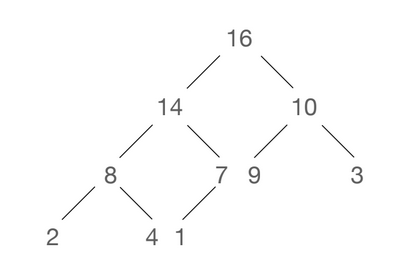
\includegraphics[width=6cm]{images/heap_tree.png}
		\caption{Albero binario quasi completo}
	\end{subfigure}
	\begin{subfigure}{.5\textwidth}
		\centering
		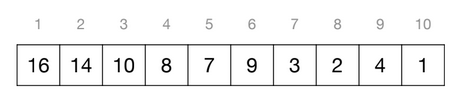
\includegraphics[width=6cm]{images/heap_array.png}
		\caption{Heap}
	\end{subfigure}
\end{figure}

\noindent
Di seguito alcune formule utili:
\begin{itemize}
	\item parent(i) = $\lfloor i/2 \rfloor$
	\item left(i) = $2i$
	\item right(i) = $2i+1$
\end{itemize}

\subsection{Max e min heap}
Dato un heap, se gli elementi di ogni sotto-albero sono più piccoli della radice del sotto-albero, allora abbiamo un \textbf{max-heap} e il massimo valore sarà memorizzato sempre nella radice.
\begin{equation}
	\forall i \neq 1, A[parent(i)] \geq A[i]
\end{equation}
Analogamente per il \textbf{min-heap} il minimo valore sarà nella radice.
\begin{equation}
	\forall i \neq 1, A[parent(i)] \leq A[i]
\end{equation}

\subsection{Proprietà}
\begin{itemize}
	\item \textbf{Proprietà 1}: un \textit{heap} di $n$ elementi ha altezza $\theta(\log{n})$, precisamente \color{red} $\lfloor \log{n} \rfloor$ \color{black}
	\item \textbf{Proprietà 2}: un \textit{heap} di $n$ elementi contiene \color{red} $\lceil n/2 \rceil$ \color{black} foglie
	\item \textbf{Proprietà 3}: un \textit{heap} di $n$ elementi ha al più \color{red} $\lceil n/2^{h+1} \rceil$ \color{black} nodi di altezza $h$, esattamente $\lceil n/2^{h+1} \rceil$ se è un albero \textit{bilanciato completo}
\end{itemize}
% !TeX spellcheck = it_IT
\newpage

\section{Algoritmi}
\subsection{Divide et impera}
È una tecnica di risoluzione di problemi che consiste in tre passi:
\begin{itemize}
	\item \textbf{Dividere} il problema in 2 o più sotto problemi identici ma di dimensione ridotta rispetto a quello originale
	\item \textbf{Risolvere} i sotto problemi \emph{ricorsivamente}
	\item \textbf{Combinare} le soluzioni dei sotto problemi per ottenere la soluzione del problema iniziale
\end{itemize}
\subsection{Ordinamento}
\begin{definition}[Algoritmo stabile]
	Un algoritmo di ordinamento si dice stabile quando preserva l'ordine iniziale tra due elementi con la stessa chiave.
\end{definition}
\subsubsection{Merge sort}
L'idea è di usare la tecnica precedentemente descritta del \textbf{Divide et Impera} e di spezzare l'array in due sotto-array di uguale dimensione, ordinarli e poi fonderli in uno unico. \\
La fusione verrà fatta confrontando i primi due elementi di ogni sotto-array, copiando il più piccolo nell'array finale, e proseguendo con il confronto del più grande con il successivo.
\begin{figure}[h]
	\begin{subfigure}{.5\textwidth}
		\centering
		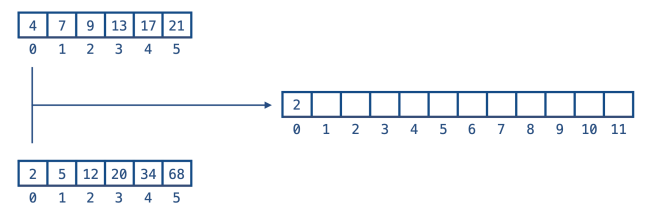
\includegraphics[width=8cm]{images/mergesort_1.png}
	\end{subfigure}
	\begin{subfigure}{.5\textwidth}
		\centering
		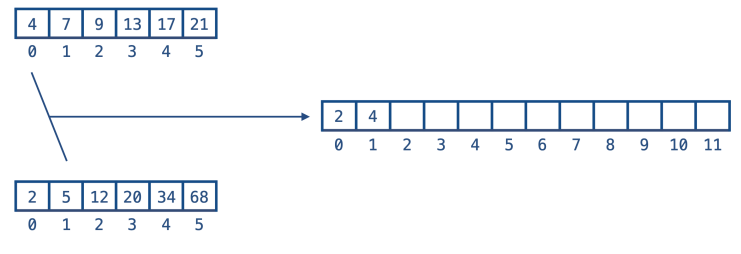
\includegraphics[width=8cm]{images/mergesort_2.png}
	\end{subfigure}
\end{figure}
\begin{figure}[h]
	\begin{subfigure}{.5\textwidth}
		\centering
		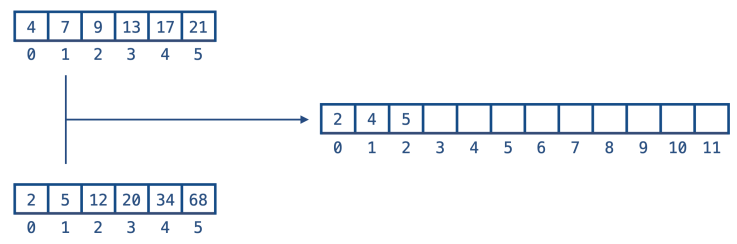
\includegraphics[width=8cm]{images/mergesort_3.png}
	\end{subfigure}
	\begin{subfigure}{.5\textwidth}
		\centering
		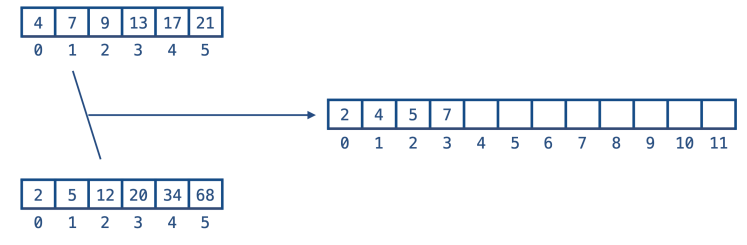
\includegraphics[width=8cm]{images/mergesort_4.png}
	\end{subfigure}
\end{figure}

\noindent Esempio di implementazione:

\begin{lstlisting}[language=C, caption=Algoritmo merge sort, mathescape=true]
	void merge_sort(int a[], size_t dim, char order) {
		sort(a, 0, dim-1, order);
	}

	void sort(int a[], size_t inizio, size_t fine, char order) {
		if ((fine - inizio) >= 1) {
			// Passo ricorsivo
			size_t centro1 = (inizio + fine)/2;
			zie_t centro2 = centro1 + 1;
			
			sort(a, inizio, centro1, order);
			sort(a, centro2, fine, order);
			
			merge(a, inizio, centro1, centro2, fine, order);
		}
		// Il caso base non serve, un array di un elemento e' ordinato
	}
	
	void merge(int a[], size_t sin, size_t centro1, size_t centro2, size_t dx, char order) {
		size_t sin i = sin;
		size_t dx_i = centro2;
		size_t fondi i = 0;
		int temp_a[dx - sin + 1];
		
		while (sin_i <= centro1 && dx_i <= dx) {
			switch (order) {
				case 'I':				
					if (a[sin_i] <= a[dx_i]) {
						temp_a[fondi_i++] = a[sin_i++];
					} else {
						temp_a[fondi_i++] = a[dx_i++];
					}
					break;
				default:
					if (a[sin_i] <= a[dx_i]) {
						temp_a[fondi_i++] = a[dx_i++];
					} else {
						temp_a[fondi_i++] = a[sin_i++];
					}
					break;
			}
		}
		
		// Se esaurisco il sotto-array sinistro
		if (sin_i == centro2) {
			while (dx_i <= dx) {
				temp_a[fondi_i++] = a[dx_i++];
			}
		} else {
			// Se esaurisco quello destro
			while (sin_i <= centro1) {
				temp_a[fondi_i++] = a[sin_i++];
			}
		}
	
		// Copio l'array temporaneo in quello originale
		for (size_t i = sin; i <= dx; i++) {
			a[i] = temp_a[i-sin];	
		}
	}
\end{lstlisting}

\subsubsection{Insertion sort}
\textbf{Proprietà}: al termine del passo j-esimo dell'algoritmo l'elemento j-esimo viene in inserito al posto giusto e i primi $j+1$ elementi sono ordinati.
\begin{lstlisting}[language=Javascript, caption=Algoritmo insertion sort, mathescape=true]
	insertionSort(A) =
	var j:Int = 0;
	var i:Int = 0;		$\Theta(1)$
	var k:int = 0;
	for (j=1; j<n; j++) {		$n-1$ volte
		k = A[j];
		i = j-1;		$\Theta(1)$ $n-1$ volte
		while(i >= 0 && A[i]>k) {
			A[i+1] = A[i];			$\Theta(1)$ $\sum\limits_{j=1}^{n-1} (t_j-1)$ volte
			i=i-1;
		}
		A[i+1] = k;		$\Theta(1)$ $n-1$ volte
	}
\end{lstlisting}

\begin{table}[h]
	\centering
	\begin{tabular}{ |c|c|c|c|c|c| }
		\hline
		0 & 1 & 2 & 3 & 4 & 5 \\
		\hline
		5 & 2 & 4 & 6 & 1 & 3 \\
		\hline 
		5 & 2 & 4 & 6 & 1 & 3 \\
		\hline 
		5 & 5 & 4 & 6 & 1 & 3 \\
		\hline 
		2 & 5 & 4 & 6 & 1 & 3 \\
		\hline 
		2 & 5 & 4 & 6 & 1 & 3 \\
		\hline 
		2 & 5 & 5 & 6 & 1 & 3 \\
		\hline 
		2 & 4 & 5 & 6 & 1 & 3 \\
		\hline 
		2 & 4 & 5 & 6 & 1 & 3 \\
		\hline 
		2 & 4 & 5 & 6 & 1 & 3 \\
		\hline 
	\end{tabular}
	\begin{tabular} { |c|c|c|c|}
		\hline
		j & i & k & while \\
		\hline
		0 & 0 & 0 & no \\
		\hline
		1 & 0 & 2 & si \\
		\hline
		1 & -1 & 2 & no \\
		\hline
		1 & -1 & 2 & no \\
		\hline
		2 & 1 & 4 & si \\
		\hline
		2 & 0 & 4 & no \\
		\hline
		2 & 0 & 4 & no \\
		\hline
		3 & 2 & 6 & no \\
		\hline
		3 & 2 & 6 & no \\
		\hline
	\end{tabular}
	\caption{Esempio di esecuzione}
\end{table}
\textbf{Complessità}:
\begin{align*}
	\sum\limits_{j=1}^{n-1} t_j
\end{align*}
\begin{itemize}
	\item Caso pessimo: l'array è ordinato decrescente e quindi ogni volta devo scalare l'elemento fino alla prima posizione. Abbiamo che $t_j = j$ e $\sum\limits_{j=1}^{n-1} j = \frac{n(n-1)}{2}$, quindi $O(n^2)$
	\item Caso migliore: l'array è ordinato crescente e quindi per ogni iterazione non entro nel while perché la condizione è falsa. Abbiamo $t_j = 1$ e $\sum\limits_{j=1}^{n-1} j = n-1$, quindi $O(n)$
	\item Caso medio: come il caso pessimo $O(n^2)$
\end{itemize}
\textbf{Correttezza}:
\begin{itemize}
	\item dimostro l'\textbf{invariante di ciclo} per assicurarmi che la mia proprietà venga mantenuta durante tutta l'esecuzione. Lo faccio tramite \emph{induzione}:
	\begin{itemize}
		\item Caso base: per $j=1$
		\item Hp induttiva: per $j=n'$
		\item Passo induttivo: dimostro che vale anche per $j=n'+1$
	\end{itemize}
	\item verifico la \textbf{terminazione}: il \emph{for} è eseguito esattamente $n-1$ volte e il \emph{while} al più $j-1$ volte, quindi tutte le iterazioni sono finite e l'algoritmo termina.
\end{itemize}
\textbf{Memoria impiegata}: ordina in loco quindi non usa memoria aggiuntiva.

\subsubsection{Selection sort}
\textbf{Proprietà}: al termine del passo j-esimo dell'algoritmo i primi $j+1$ elementi di A sono ordinati e contengono i $j+1$ elementi più piccoli di A.
%TODO Calcolo della complessità non corretto
\begin{lstlisting}[language=Javascript, caption=Algoritmo selection sort, mathescape=true]
	insertionSort(A) =
	var j:Int = 0;
	var i:Int = 0;		$\Theta(1)$
	var min:int = 0;
	for (i=0; i<n-1; i++) {		$n-1$ volte
		min = i;		$\Theta(1)$ $n-1$ volte
		for(j=i+1; j<n; j++) {
			if A[j] < A[min] {min = j};			$\Theta(1)$ $\sum\limits_{j=1}^{n-1} (t_j-1)$ volte
		}
		swap(A[i],A[min]);		$\Theta(1)$ $n-1$ volte
	}
\end{lstlisting}
\begin{table}[h]
	\centering
	\begin{tabular}{ |c|c|c|c|c|c| }
		\hline
		0 & 1 & 2 & 3 & 4 & 5 \\
		\hline
		5 & 2 & 4 & 6 & 1 & 3 \\
		\hline 
		1 & 2 & 4 & 6 & 5 & 3 \\
		\hline 
		1 & 2 & 4 & 6 & 5 & 3 \\
		\hline 
		1 & 2 & 3 & 6 & 5 & 4 \\
		\hline 
		1 & 2 & 3 & 4 & 5 & 6 \\
		\hline 
		1 & 2 & 3 & 4 & 5 & 6 \\
		\hline
	\end{tabular}
	\begin{tabular} { |c|c|c|}
		\hline
		j & i & min \\
		\hline
		0 & 0 & 0 \\
		\hline
		1 & 0 & 4 \\
		\hline
		2 & 1 & 1 \\
		\hline
		3 & 2 & 5 \\
		\hline
		4 & 3 & 3 \\
		\hline
		5 & 4 & 4 \\
		\hline
	\end{tabular}
	\caption{Esempio di esecuzione}
\end{table}
\textbf{Complessità}
%TODO Inserisci il calcolo della complessità
\begin{align*}
	\sum\limits_{j=1}^{n-1} j = \frac{n(n-1)}{2} \in O(n^2)
\end{align*}
\begin{itemize}
	\item Caso pessimo: $O(n^2)$
	\item Caso migliore: $O(n^2)$
	\item Caso medio: $O(n^2)$
\end{itemize}
\textbf{Correttezza}:
\begin{itemize}
	\item dimostro l'\textbf{invariante di ciclo} per assicurarmi che la mia proprietà venga mantenuta durante tutta l'esecuzione. Sempre tramite induzione.
	\item verifico la \textbf{terminazione} in maniera analoga all'insertion sort.
\end{itemize}
\textbf{Memoria impiegata}: ordina in loco quindi non usa memoria aggiuntiva.

\subsubsection{Bubble sort}
Questo algoritmo scorre l'array e, a coppie, ordina gli elementi facendo più passate. Il nome \emph{bubble} deriva dal fatto che ad ogni passata i numeri più grandi (o piccoli) si spostano verso la fine dell'array come le bolle d'aria salgono a galla.
\begin{lstlisting}[language=C, caption=Algoritmo bubble sort, mathescape=true]
	void bubble_sort (int a[], size_t dim, char order) {
		int temp;
		for (unsigned int passate = 0; passate < dim; passate++) {
			for (size_t i=0; i < (dim - 1); i++) {
				switch (order) {
					case 'I':
						if (a[i] > a[i+1]) {
							temp = a[i];
							a[i] = a[i+1];
							a[i+1] = temp;
						}
						break;
					default:
						if (a[i] < a[i+1]) {
							temp = a[i];
							a[i] = a[i+1];
							a[i+1] = temp;
							 break;
						}
				}
			}
		}
	}
\end{lstlisting}
\textbf{Complessità}\\
Il primo \emph{for} esegue $n$ cicli e quello interno ne esegue $n-1$. Di conseguenza la complessità è $n\cdot (n-1)$, ovvero $\mathbf{n^2}$.
\subsection{Linear sort}
Gli algoritmi di ordinamento di questo tipo sfruttano il fatto che l'array da ordinare abbia determinate proprietà.
\begin{example}
	Dato un array $A$ di $n$ interi compresi tra $1$ e $k$:
	\begin{align*}
		\forall 0 < j \leq n . A[j] \in [1, \ldots, k]
	\end{align*}
	\begin{lstlisting}[language=Javascript, caption=Algoritmo linear sort, mathescape=true]
		linearSort(A:[Int], B:[Int], k:Int) -> Void {
			// Inizializzo un array che tiene conto dei numeri da 1 a k
			for (var i:Int = 1; i<=k; i++) C[i] = 0;	$\Theta(k)$
			
			var j:Int = 1;
			// Conto quante volte compare ogni numero nell'array originale
			for (j=1; j<=n; j++) C[A[j]] += 1;	$\Theta(n)$
				
			j=1;
			var z:Int = 1;
			// Dispongo ogni numero nell'array finale in ordine sapendo quante volte compare
			for (z=1; z <= k; z++) {	$\Theta(k)$
				for (var v:Int = 0; v < C[z]; v++) {	$\Theta(n)$
					B[j] = z;
					j++;	
				}	
			}	
		}
	\end{lstlisting}
	\textbf{Complessità}\\
	In questo caso la complessità è $\Theta(n + k)$ e si usa quando $k \in O(n)$.
\end{example}
\subsubsection{Radix sort}
Questo algoritmo funziona in maniera simile a come il cervello umano ordina gruppi di numeri: si ordinano (tramite un algoritmo di ordinamento \textbf{stabile} prima le cifre delle migliaia, poi quelle delle centinaia, quelle delle decine ed infine le unità. Notiamo però che il risultato NON è corretto.
\begin{table}[h]
	\centering
	\begin{tabular}{ccccc}
		\textbf{1}094 & \textbf{9}86 & 10\textbf{9}4 & 12\textbf{5} & 1120 \\
		986 & \textbf{2}34 & 1\textbf{2}5 & 112\textbf{0} & 234 \\
		234 & \textbf{1}25 & 11\textbf{2}0 & 23\textbf{4} & 1094 \\
		125 & 1\textbf{0}94 & 2\textbf{3}4 & 98\textbf{6} & 125 \\
		\textbf{1}120 & 1\textbf{1}20 & 9\textbf{8}6 & 109\textbf{4} & 986
	\end{tabular}
\end{table}
\\
Per farlo funzionare dobbiamo ordinare le cifre partendo da quelle meno significative, quindi dalle unità.
\begin{table}[h]
	\centering
	\begin{tabular}{ccccc}
		109\textbf{4} & 11\textbf{2}0 & 1\textbf{1}20& \textbf{1}094 & 125 \\
		98\textbf{6} & 10\textbf{9}4 & \textbf{1}25 & \textbf{1}120 & 234 \\
		23\textbf{4} & 2\textbf{3}4 & \textbf{2}34 & 125 & 986 \\
		12\textbf{5} & 1\textbf{2}5 & \textbf{9}86 & 234 & 1094 \\
		112\textbf{0} & 9\textbf{8}6 & 1\textbf{0}94 & 986 & 1120
	\end{tabular}
\end{table}
\section{Complessità}
\subsection{Limiti inferiori}
\subsubsection{Complessità di un problema}
Per determinare il limite inferiore di un problema al caso pessimo, analizzo le seguenti cose:
\begin{itemize}
	\item \textbf{Dimensione dei dati}: Se la soluzione di un problema richiede l'esame di tutti i dati in input, allora $\Omega(n)$ è un limite inferiore. \emph{E.g. sommare tutti gli elementi di un array.}
	\item \textbf{Eventi contabili}: se la soluzione di un problema richiede la ripetizione di un certo evento, allora il numero di volte che l'evento si ripete (moltiplicato per il suo costo) è un limite inferiore.
	\item \textbf{Alberi di decisione}: sono alberi in cui
	\begin{itemize}
		\item ogni nodo non foglia effettua un test su un attributo
		\item ogni arco uscente da un nodo è un possibile valore dell'attributo
		\item ogni nodo foglia assegna una classificazione
	\end{itemize}
	Si applica a problemi risolubili attraverso sequenze di decisioni che via via riducono lo spazio delle soluzioni.
	%TODO inserire immagine di albero di decisione
	\begin{note}
		Alcune formule importanti per gli alberi:
		%TODO Inserisci formule
	\end{note}
	%TODO Esempio con ricerca binaria
\end{itemize}

\subsubsection{Ordinamento}
\subsubsection{Insertion sort}
\textbf{Proprietà}: al termine del passo j-esimo dell'algoritmo l'elemento j-esimo viene in inserito al posto giusto e i primi $j+1$ elementi sono ordinati.
\begin{lstlisting}[language=Javascript, caption=Algoritmo insertion sort, mathescape=true]
	insertionSort(A) =
	var j:Int = 0;
	var i:Int = 0;		$\Theta(1)$
	var k:int = 0;
	for (j=1; j<n; j++) {		$n-1$ volte
		k = A[j];
		i = j-1;		$\Theta(1)$ $n-1$ volte
		while(i >= 0 && A[i]>k) {
			A[i+1] = A[i];			$\Theta(1)$ $\sum\limits_{j=1}^{n-1} (t_j-1)$ volte
			i=i-1;
		}
		A[i+1] = k;		$\Theta(1)$ $n-1$ volte
	}
\end{lstlisting}
\begin{table}[h]
	\begin{tabular}{ |c|c|c|c|c|c| }
		\hline
		0 & 1 & 2 & 3 & 4 & 5 \\
		\hline
		5 & 2 & 4 & 6 & 1 & 3 \\
		\hline 
		5 & 2 & 4 & 6 & 1 & 3 \\
		\hline 
		5 & 5 & 4 & 6 & 1 & 3 \\
		\hline 
		2 & 5 & 4 & 6 & 1 & 3 \\
		\hline 
		2 & 5 & 4 & 6 & 1 & 3 \\
		\hline 
		2 & 5 & 5 & 6 & 1 & 3 \\
		\hline 
		2 & 4 & 5 & 6 & 1 & 3 \\
		\hline 
		2 & 4 & 5 & 6 & 1 & 3 \\
		\hline 
		2 & 4 & 5 & 6 & 1 & 3 \\
		\hline 
	\end{tabular}
	\begin{tabular} { |c|c|c|c|}
		\hline
		j & i & k & while \\
		\hline
		0 & 0 & 0 & no \\
		\hline
		1 & 0 & 2 & si \\
		\hline
		1 & -1 & 2 & no \\
		\hline
		1 & -1 & 2 & no \\
		\hline
		2 & 1 & 4 & si \\
		\hline
		2 & 0 & 4 & no \\
		\hline
		2 & 0 & 4 & no \\
		\hline
		3 & 2 & 6 & no \\
		\hline
		3 & 2 & 6 & no \\
		\hline
	\end{tabular}
	\caption{Esempio di esecuzione}
\end{table}
\textbf{Complessità} bla bla bla\\ %TODO Inserisci il calcolo della complessità
\textbf{Correttezza}:
\begin{itemize}
	\item dimostro l'\textbf{invariante di ciclo} per assicurarmi che la mia proprietà venga mantenuta durante tutta l'esecuzione. Lo faccio tramite \emph{induzione}:
	\begin{itemize}
		\item Caso base: per $j=1$
		\item Hp induttiva: per $j=n'$
		\item Passo induttivo: dimostro che vale anche per $j=n'+1$
	\end{itemize}
	\item verifico la \textbf{terminazione}: il \emph{for} è eseguito esattamente $n-1$ volte e il \emph{while} al più $j-1$ volte, quindi tutte le iterazioni sono finite e l'algoritmo termina.
\end{itemize}
\textbf{Memoria impiegata}: ordina in loco quindi non usa memoria aggiuntiva.

\subsubsection{Selection sort}
\textbf{Proprietà}: al termine del passo j-esimo dell'algoritmo i primi $j+1$ elementi di A sono ordinati e contengono i $j+1$ elementi più piccoli di A.
\begin{lstlisting}[language=Javascript, caption=Algoritmo selection sort, mathescape=true]
	insertionSort(A) =
	var j:Int = 0;
	var i:Int = 0;		$\Theta(1)$
	var min:int = 0;
	for (i=0; i<n-1; i++) {		$n-1$ volte
		min = i;		$\Theta(1)$ $n-1$ volte
		for(j=i+1; j<n; j++) {
			if A[j] < A[min] {min = j};			$\Theta(1)$ $\sum\limits_{j=1}^{n-1} (t_j-1)$ volte
		}
		swap(A[i],A[min]);		$\Theta(1)$ $n-1$ volte
	}
\end{lstlisting}
\begin{table}[h]
	\begin{tabular}{ |c|c|c|c|c|c| }
		\hline
		0 & 1 & 2 & 3 & 4 & 5 \\
		\hline
		5 & 2 & 4 & 6 & 1 & 3 \\
		\hline 
		1 & 2 & 4 & 6 & 5 & 3 \\
		\hline 
		1 & 2 & 4 & 6 & 5 & 3 \\
		\hline 
		1 & 2 & 3 & 6 & 5 & 4 \\
		\hline 
		1 & 2 & 3 & 4 & 5 & 6 \\
		\hline 
		1 & 2 & 3 & 4 & 5 & 6 \\
		\hline
	\end{tabular}
	\begin{tabular} { |c|c|c|}
		\hline
		j & i & min \\
		\hline
		0 & 0 & 0 \\
		\hline
		1 & 0 & 4 \\
		\hline
		2 & 1 & 1 \\
		\hline
		3 & 2 & 5 \\
		\hline
		4 & 3 & 3 \\
		\hline
		5 & 4 & 4 \\
		\hline
	\end{tabular}
	\caption{Esempio di esecuzione}
\end{table}
\textbf{Complessità}
%TODO Inserisci il calcolo della complessità
\begin{equation}
	\sum\limits_{j=1}^{n-1} j = \frac{n(n-1)}{2} \in O(n^2)
\end{equation}
\begin{itemize}
	\item Caso pessimo: $O(n^2)$
	\item Caso migliore: $O(n^2)$
	\item Caso medio: $O(n^2)$
\end{itemize}
\textbf{Correttezza}:
\begin{itemize}
	\item dimostro l'\textbf{invariante di ciclo} per assicurarmi che la mia proprietà venga mantenuta durante tutta l'esecuzione. Sempre tramite induzione.
	\item verifico la \textbf{terminazione} in maniera analoga all'insertion sort.
\end{itemize}
\textbf{Memoria impiegata}: ordina in loco quindi non usa memoria aggiuntiva.
% !TeX spellcheck = it_IT
\newpage
\section{Liste}
Una \textbf{struct} (struttura) \textbf{autoreferenziale} ha un membro puntatore che punta a una struttura dello stesso tipo, chiamato \textbf{link}, e che serve a creare una \emph{catena} (lista) di nodi collegati tra loro.
\begin{lstlisting}[language=C, caption=Esempio di una struct]
	struct nodo {
		int dato;
		struct nodo *nextPtr;
	} n1, n2, n3;
\end{lstlisting}

\begin{definition}[Struttura dinamica]
	È una struttura dati che può \textbf{variare} la sua dimensione a tempo di esecuzione, aumentando e diminuendo. Alcuni esempi sono proprio le \textbf{liste}, oltre che le pile, le code e gli alberi binari.
\end{definition}

\begin{note}
	L'ultimo nodo di una lista conterrà nel link \textbf{null}.
\end{note}

\subsection{Confronto tra liste e array}
\begin{table}[!h]
	\centering
	\begin{tabular}{|p{150px}|p{150px}|}
		\hline
		\textbf{Liste} & \textbf{Array} \\
		\hline
		Contiene sequenze di dati & Contiene sequenze di dati \\ 
		\hline
		Create dinamicamente a tempo di esecuzione e la dimensione non può essere prevista a tempo di compilazione & Creati staticamente a tempo di esecuzione e la dimensione deve essere calcolabile a tempo di compilazione \\
		\hline
		La dimensione è variabile &  La dimensione è costante e tutti gli elementi sono allocati a tempo di definizione\\
		\hline
		Diventa piena solo quando termina la memoria disponibile nell'heap & Diventa pieno quando sono pieni tutti gli elementi \\
		\hline
		Non sono memorizzate in celle contigue & Sono in celle contigue \\
		\hline
		Possono essere manipolate senza spostare elementi & Per manipolarli bisogna spostare gli elementi \\
		\hline
	\end{tabular}
\end{table}

\subsection{Operazioni sulle liste}
\subsubsection{Insert}
Viene codificata come segue:
\begin{lstlisting}[language=C, caption=Inserimento in una lista]
	void insert(NodoPtr *lPtr, int val) {
		// Alloco nuovo nodo
		NodoPtr nuovoPtr = malloc(sizeof(Nodo));
		if (nuovoPtr != NULL) {
			// Inizializzo nodo
			nuovoPtr->dato = val;
			nuovoPtr->prossimoPtr = NULL;
			NodoPtr precedentePtr = NULL;
			NodoPtr correntePtr = *lPtr;
			while (correntePtr != NULL && val > correntePtr->dato) {
				precedentePtr = correntePtr;
				correntePtr = correntePtr->prossimoPtr;
			}
			if (precedentePtr == NULL) {
				// Inserimento all'inizio della lista
				nuovoPtr->prossimoPtr = *lPtr;
				*lPtr = nuovoPtr;
			}
			else {
				// Inserimento tra due nodi
				precedentePtr->prossimoPtr = nuovoPtr;
				nuovoPtr->prossimoPtr = correntePtr;
			}
		}
		else {
			puts("Memoria esaurita");
		}
	}
\end{lstlisting}

\subsubsection{Delete}
Viene codificata come segue:
\begin{lstlisting}[language=C, caption=Cancellazione in una lista]
void delete(NodoPtr *lPtr, int val) {
	if (*lPtr != NULL) {
		if (val == (*lPtr)->dato) {
			NodoPtr tempPtr = *lPtr;
			*lPtr = (*lPtr)->prossimoPtr;
			free(tempPtr);
		}
		else {
			NodoPtr precedentePtr = *lPtr;
			NodoPtr correntePtr = (*lPtr)->prossimoPtr;
			while (correntePtr != NULL && correntePtr->dato != val) {
				precedentePtr = correntePtr;
				correntePtr = correntePtr->prossimoPtr;
			}
			if (correntePtr != NULL) {
				NodoPtr tempPtr = correntePtr;
				precedentePtr->prossimoPtr = correntePtr->prossimoPtr;
				free(tempPtr);
			}
		}
	}
}
\end{lstlisting}

\subsubsection{Verifica se è vuota}
\begin{lstlisting}[language=C, caption=Verificare se la lista è vuota]
int is_empty(NodoPtr lPtr) {
	return lPtr == NULL;
}
\end{lstlisting}

\subsection{Liste particolari}
\subsubsection{Pile}
\begin{definition}
	Una \textbf{pila} è una lista in cui inserimenti e cancellazioni possono essere fatte solo sulla testa della lista (politica \textbf{LIFO}).
\end{definition}
Le operazioni che possono essere eseguite sulle pile sono:
\begin{itemize}
	\item \textbf{Push}: inserimento di un nuovo nodo in testa
	\begin{lstlisting}[language=C]
		void push(NodoPtr *topPtr, int val) {
			// alloco nuovo nodo
			NodoPtr nuovoPtr = malloc(sizeof(Nodo));
			if (nuovoPtr != NULL) { // Spazio disponibile
				// inizializzo nodo
				nuovoPtr->dato = val;
				nuovoPtr->prossimoPtr = *topPtr;
				*topPtr = nuovoPtr;
			}
			else {
				puts("Memoria esaurita");
			}
		}
	\end{lstlisting}
	\item  \textbf{Pop}: cancellazione di un elemento in testa
	\begin{lstlisting}[language=C]
		int pop(NodoPtr *topPtr) {
			int val = (*topPtr)->dato;
			NodoPtr tempPtr = *topPtr;
			*topPtr = (*topPtr)->prossimoPtr;
			free(tempPtr);
			return val;
		}
	\end{lstlisting}
	\item \textbf{is\_empty}, \textbf{stampa\_pila}
\end{itemize}

\subsubsection{Code}
\begin{definition}
	Una \textbf{pila} è una lista in cui inserimenti e cancellazioni possono essere fatte solo alla fine della lista (politica \textbf{FIFO}).
\end{definition}
Le operazioni che possono essere eseguite sulle pile sono:
\begin{itemize}
	\item \textbf{Enqueue}: inserimento di un nuovo nodo alla fine della coda
	\begin{lstlisting}[language=C]
		void enqueue(NodoPtr *testaPtr, NodoPtr * codaPtr, int val) {
			// alloco nuovo nodo
			NodoPtr nuovoPtr = malloc(sizeof(Nodo));
			if (nuovoPtr != NULL) { // Spazio disponibile
				// inizializzo nodo
				nuovoPtr->dato = val;
				nuovoPtr->prossimoPtr = NULL;
				if (is_empty(*testaPtr)) {
					*testaPtr = nuovoPtr;
				}
				else {
					(*codaPtr)->prossimoPtr = nuovoPtr;
					*codaPtr = nuovoPtr;
				}
			}
			else {
				puts("Memoria esaurita");
			}
		}
	\end{lstlisting}
	\item  \textbf{Dequeue}: cancellazione di un elemento in testa
	\begin{lstlisting}[language=C]
		int dequeue(NodoPtr *testaPtr, NodoPtr * codaPtr) {
			int val = (*testaPtr)->dato;
			NodoPtr tempPtr = *testaPtr;
			*testaPtr = (*testaPtr)->prossimoPtr;	
			if (*testaPtr == NULL) {
				*codaPtr = NULL;
			}
			free(tempPtr);
			return val;
		}
	\end{lstlisting}
	\item \textbf{is\_empty}, \textbf{stampa\_coda}
\end{itemize}
\end{document}